% !TEX root =  free222.tex
\chapter{Methods of Integration} %{{{1
\label{cha:integrals}
The basic question that this chapter addresses is how to compute integrals, i.e.
\begin{center}
  \itshape Given a function $y=f(x)$ how do we find\\
  a function $y=F(x)$ whose derivative is $F'(x) = f(x)$?
\end{center}
The simplest solution to this problem is to look it up on the Internet.  Any
integral that we compute in this chapter can be found by typing it into the
following web page:
\begin{center}
  \url{http://integrals.wolfram.com}
\end{center}
Other similar websites exist, and more extensive software packages are
available.

It is therefore natural to ask \textit{why should we learn how to do these
  integrals?}  The question has at least two answers.

First, there are certain \textit{basic integrals} that show up frequently and
that are relatively easy to do (once we know the trick), but that are not
included in a first semester calculus course for lack of time.  Knowing these
integrals is useful in the same way that knowing things like ``$2+3=5$'' saves
us from a lot of unnecessary calculator use.

\def\electroniccircuitoutput%
{\parbox{120pt}
{\centering Output signal\\$\DS g(t) = \int_0^t e^{\tau-t} f(\tau)\,\dd \tau$}}
\def\electroniccircuitinput%
{\parbox{75pt}{\centering Input signal\\$f(t)$}}
\footnotesize\sffamily
\vspace{4ex}
\input ../figures/222/01electroniccircuit.pdf_tex
\normalsize\rmfamily

The second reason is that we often are not really interested in
specific integrals, but in general facts about integrals.  For
example, the output $g(t)$ of an electric circuit (or mechanical
system, or a biochemical system, etc.) is often given by some integral
involving the input $f(t)$.  The methods of integration that we will see in
this chapter give us the tools we need to understand why some integral
gives the right answer to a given electric circuits problem, no matter
what the input $f(t)$ is.


\section{Definite and indefinite integrals} %{{{1
\label{sec:the-indefinite-integral}
We recall some facts about integration from first semester calculus.
\begin{definition}
  A function $y=F(x)$ is called an \emph{antiderivative} of another function
  $y=f (x)$ if $F'(x)=f(x)$ for all $x$.
\end{definition}
\medskip

For instance, $F(x) = \frac12 x^2$ is an antiderivative of $f(x) = x$, and so is
$G(x) = \frac12x^2+2012$.

The \emph{Fundamental Theorem of Calculus} states that if a function $y=f(x)$ is
continuous on an interval $a\leq x\leq b$, then there always exists an
antiderivative $F(x)$ of $f$, and one has
\begin{equation}
  \label{eq:01FundamentalTheorem}
  \int_a^b f(x)\,\dd x =F(b)-F(a).
\end{equation}
For example, if $f(x) = x$, then $F(x) = \frac12x^2$ is an antiderivative for
$f(x)$, and thus $\int_a^b x\,\dd x = F(b)-F(a) = \frac12b^2 -\frac12a^2$.

The best way of computing an integral is often to find an antiderivative $F$ of
the given function $f$, and then to use the Fundamental Theorem
(\ref{eq:01FundamentalTheorem}).  \textit{How to go about finding an
  antiderivative $F$ for some given function $f$ is the subject of this
  chapter.}

The following notation is commonly used for antiderivatives:
\begin{equation}
  \label{eq:2}
  F(x) = \int f(x) \dd x .
\end{equation}
The integral that appears here does not have the integration bounds $a$ and
$b$. It is called an \emph{indefinite integral}, as opposed to the integral in
(\ref{eq:01FundamentalTheorem}) which is called a \emph{definite integral}. It
is important to distinguish between the two kinds of integrals.
Table~\ref{tbl:01definite-versus-indefinite} lists the main differences.
\smallskip

\begin{table}[t]\sffamily
  \color[rgb]{0,0.25,0.5}%
  \begin{tabular}{@{\extracolsep{2em}}cc}
    \toprule[2pt]
    \bfseries Indefinite integral & \bfseries Definite integral\\[2pt]
      \midrule \\ \color{darkgreen}
    $\int f(x) d x$ is a function of $x$.&
    \color{darkgreen}
    $\int_a^bf(x)d x$ is a number. \\[4ex]
    \begin{minipage}[t]{160pt}
      By definition $\int f(x)d x$ is \textit{any function $F(x)$ whose
        derivative is $f(x)$. }
    \end{minipage} &
    \begin{minipage}[t]{160pt}
      $\int_a^b f(x)d x$ was defined in terms of Riemann sums and can be
      interpreted as ``area under the graph of $y=f(x)$'' when $f(x) \geq 0$.
      \vspace{2ex}
    \end{minipage}
    \\[8ex]
    \begin{minipage}[t]{160pt}\color{darkgreen}
      If $F(x)$ is an antiderivative of $f(x)$, then so is $F(x)+C$.  Therefore
      $\int f(x)\dd x = F(x)+C$; an indefinite integral contains a constant
      (``$+C$'').  \vspace{2ex}
    \end{minipage} &
    \begin{minipage}[t]{160pt}\color{darkgreen}
      $\int_a^b f(x)d x$ is one uniquely defined number; an indefinite integral
      does not contain an arbitrary constant.
    \end{minipage}
    \\[10ex]
    \begin{minipage}[t]{160pt}
      $x$ is not a dummy variable, for example, \ $\int 2xd x=x^2+C$ and $\int
      2td t=t^2+C$ are functions of different variables, so they are not equal.
      (See Problem~\ref{pblm:01indefinite-integrals}.)
    \end{minipage}
    &    
    \begin{minipage}[t]{160pt}
      $x$ is a dummy variable, for example,
      \[\textstyle
      \int_0^1 2xd x=1, \text{ and } \int_0^1 2td t=1,
      \]
      so
      \[\textstyle
      \int_0^1 2xd x=\int_0^1 2td t.
      \]
      Whether we use $x$ or $t$ the integral makes no difference.
      \rule[-6pt]{1pt}{0pt}
    \end{minipage}
    \\[1ex]
    \bottomrule[2pt]

  \end{tabular}
  \smallskip
  \caption{Important differences between definite and indefinite integrals}
  \label{tbl:01definite-versus-indefinite}
\end{table}

% \subsection{Examples} By directly differentiating we can verify the following: %{{{2

% \begin{itemize}
% \item $F_1(x) = x^2$ is an antiderivative of $f(x)=2x$, and therefore we write
%   \[
%   \int 2x\dd x = x^2 +C.
%   \]

% \item $F_2(x) = x^2 +2004$ is also an antiderivative of $f(x)=2x$.

% \item $G(t)= \frac12\sin (2t+1)$ is an antiderivative of $g(t)=\cos (2t+1)$,
%   so
%   \[
%   \int \cos(2t+1)\; \dd t = \frac12\sin(2t+1) + C.
%   \]
% \end{itemize}

\newpage

\section{Problems} %{{{1

\problemfont %{{{3
\begin{multicols}{2}
\problem Compute the following integrals: %{{{3
\label{pblm:01indefinite-integrals}

\subprob $A=\int x^{-2} \,\dd x,$
\answer %{{{3
$A = -x^{-1}+C$,
\endanswer

\subprob $B=\int t^{-2} \,\dd t,$
\answer %{{{3
$B = -t^{-1}+C$,
\endanswer

\subprob $C=\int x^{-2} \,\dd t,$
\answer %{{{3
$C = tx^{-2}+C$,
\endanswer

\subprob $I= \int xt \,\dd t,$
\answer %{{{3
$I = \frac12 xt^2 + C$, $J = \frac12 x^2t+C$.
\endanswer

\subprob $J= \int xt\,\dd x.$


\problem One of the following three integrals is not the same as %{{{3
the other two:
\begin{align*}
  A&=\int^4_{1} x^{-2} \,\dd x,\\
  B&=\int^4_{1} t^{-2} \,\dd t,\\
  C&=\int^4_{1} x^{-2} \,\dd t.
\end{align*}
Which one?  Explain your answer.
\columnbreak

\problem Which of the following inequalities are true? %{{{3

\subprob $\DS \int_2^4 (1-x^2) \dd x > 0$

\subprob $\DS \int_2^4 (1-x^2) \dd t > 0$

\subprob $\DS\int (1+x^2) \dd x >0$

\problem One of the following statements is correct.  Which one, and why? %{{{3

\subprob $\DS  \int_0^x 2t^2 \dd t = \tfrac23 x^3$. 

\subprob $\DS \int 2t^2 \dd t = \tfrac23 x^3$.

\subprob $\DS \int 2t^2 \dd t = \tfrac23 x^3+C$.
\end{multicols}
\noproblemfont

\section{First trick: using the double angle formulas} %{{{1
\label{sec:01double-angle-trick}
The first method of integration we see in this chapter uses trigonometric
identities to rewrite functions in a form that is easier to integrate.  This
particular trick is useful in certain integrals involving trigonometric
functions and while these integrals show up frequently, the ``double angle
trick'' is not a general method for integration.

\subsection{The double angle formulas} %{{{2
The simplest of the trigonometric identities are the double angle formulas.
These can be used to simplify integrals containing either $\sin^2 x$ or $\cos^2
x$.

Recall that
\[
\cos^2 \alpha-\sin^2\alpha = \cos 2\alpha \quad\text{ and }\quad \cos^2\alpha +
\sin^2\alpha =1,
\]
Adding these two equations gives
\[
\cos^2 \alpha =\frac12\left(\cos2\alpha+1\right)
\]
while subtracting them gives
\[
\sin^2 \alpha = \frac 12 \left(1-\cos2\alpha\right).
\]
These are the two double angle formulas that we will use.

\subsubsection{Example} The following integral shows up in many contexts, so it
is worth knowing:
\begin{align*}
  \int \cos^2 x\,\dd x
  &= \frac12 \int (1+\cos 2x)\dd x\\
  &= \frac12 \left\{x+\frac 12 \sin 2x\right\} +C\\
  &=\frac x2 +\frac 14 \sin 2x + C.
\end{align*}
Since $\sin2x=2\sin x\cos x$ this result can also be written as
\[
\int \cos^2 x\,\dd x = \frac x2+\frac12 \sin x\cos x +C.
\]
\subsubsection{A more complicated example} If we need to find
\[
I=\int \cos^4x \; \dd x
\]
then we can use the double angle trick once to rewrite $\cos^2 x$ as
$\frac12(1+\cos 2x)$, which results in
\[
I=\int \cos^4x \; \dd x
=\int\bigl\{\frac12(1+\cos 2x)\bigr\}^2 \;\dd x
=\frac14 \int \bigl(1+2\cos 2x + \cos^2 2x\bigr)\; \dd x.
\]
The first two terms are easily integrated, and now that we know the double angle
trick we also can do the third term.  We find
\[
\int\cos^2 2x\;\dd x
= \frac12 \int \bigl(1+\cos 4x\bigr)\;\dd x
= \frac x2 + \frac18\sin 4x +C.
\]
Going back to the integral $I$ we get
\begin{align*}
  I
  &= \frac14 \int \bigl(1+2\cos 2x + \cos^22x\bigr)\; \dd x\\
  &= \frac x4 + \frac14\sin 2x +\frac14 \bigl( \frac x2 + \frac 18\sin 4x\bigr) +C\\
  &= \frac {3x}8 + \frac14\sin 2x + \frac 1{32}\sin 4x +C
\end{align*}

\subsubsection{Example without the double angle trick}
The integral
\[
J=\int \cos ^3 x\;\dd x
\]
looks very much like the two previous examples, but there is very different
trick that will give us the answer.  Namely, substitute $u=\sin x$.  Then $\dd u
= \cos x \dd x$, and $\cos^2x = 1-\sin^2 x = 1-u^2$, so that
\begin{align*}
  J &= \int \cos^2 x \cos x\;\dd x \\
  &= \int (1-\sin^2 x) \cos x\;\dd x\\
  &= \int (1-u^2)\;\dd u\\
  &= u - \frac13u^3 +C \\
  &= \sin x - \frac13\sin^3 x +C.
\end{align*}

In summary, the double angle formulas are useful for certain integrals involving
powers of $\sin(\cdots)$ or $\cos(\cdots)$, but not all.  In addition to the
double angle identities there are other trigonometric identities that can be
used to find certain integrals.  See the exercises.

\section{Problems} %{{{1

\problemfont %{{{3

\begin{multicols}{2}

Compute the following integrals using the double angle formulas if necessary:

\problem $\DS\int(1+\sin2\theta)^2\, \dd \theta$ . %{{{3

\problem $\DS\int(\cos \theta+\sin\theta)^2\, \dd \theta$. %{{{3

\problem Find $\DS\int \sin^2x \cos^2x\, \dd x$\\ %{{{3
(hint: use the other double angle formula\\
$\sin2\alpha = 2\sin\alpha \cos\alpha$.)
\answer %{{{3
$ \int \sin^2x \cos^2x\, \dd
x = \frac14\int \sin^2 2x\;\dd x = \frac18\int \bigl(1-\cos 4x\bigr)\;\dd x =
\frac{x} {8} -\frac{1} {32}\sin 4x +C$.
\endanswer

\problem $\DS \int\cos^5\theta\;\dd \theta$ %{{{3
\answer Rewrite the integral as %{{{3
\[
\int \cos^5\theta\;\dd \theta = \int \cos ^4\theta\,
\underbrace{\cos\theta\;\dd\theta}_{=\dd\sin\theta}
\]
and substitute $u=\sin \theta$.  We get
\begin{align*}
  \int \cos^5\theta\;\dd \theta
  &=\int \bigl(1-u^2\bigr)^2 \;\dd u\\
  &=\int \bigl(1-2u^2+u^4\bigr)\;\dd u\\
  &=u-\frac23u^3+\frac15u^5+C\\
  &=\sin\theta -\frac23\sin^3\theta + \frac15\sin^5\theta +C.
\end{align*}
For a different solution see the section on reduction formulas.
\endanswer

\problem Find $\DS\int \Bigl(\sin^2\theta + \cos^2\theta\Bigr)^2\;\dd\theta$ %{{{3
\answer Hopefully you remembered that $\cos^2\theta+\sin^2\theta =1$.  The %{{{3
answer is $\theta+C$.
\endanswer

% \vspace{2pt} \hrule \vspace{2pt}

\noindent\itshape\color{darkbluegreen}
The double angle formulas are special cases of the following trig identities:
\begin{gather*}
  2\sin A \sin B = \cos(A-B) - \cos (A+B)\\
  2\cos A \cos B = \cos(A-B) + \cos (A+B)\\
  2\sin A \cos B = \sin(A+B) + \sin (A-B)
\end{gather*}
Use these identities to compute the following integrals.\upshape
\color{black}
\problem $\DS \int \sin x \sin 2x \ \;\dd x$ %{{{3
\answer %{{{3
Use $2\sin A \sin B = \cos(A-B) - cos (A+B)$ to rewrite the integrand as
$\sin x\sin 2x = \frac12 \bigl(\cos (x) - \cos (3x) \bigr)$.  You then get
\[
\int \sin x\sin 2x
= \frac12 \int \bigl(\cos (x) - \cos (3x) \bigr) \; \dd x
= \frac12\sin (x) - \frac16 \sin(x) + C.
\]
\endanswer

\problem $\DS \int_0^\pi \sin3x \sin 2x \ \;\dd x$ %{{{3

\problem $\DS \int \bigl(\sin 2\theta - \cos 3\theta\bigr)^2 \; \dd\theta$. %{{{3

\problem $\DS\int_0^{\pi/2} \bigl(\sin 2\theta + \sin 4\theta\bigr)^2 \;\dd %{{{3
\theta$.

\problem $\DS \int_0^\pi \sin kx \sin mx \;\dd x$ where $k$ and $m$ are constant %{{{3
positive integers.  Simplify your answer!  (careful: after working out your
solution, check if you didn't divide by zero anywhere.)


\problem Let $a$ be a positive constant and %{{{3
\[
I_a = \int_0^{\pi/2} \sin(a\theta)\cos(\theta)\,\dd \theta.
\]
\subprob Find $I_a$ if $a\ne 1$.

\subprob \carefulnow~~Find $I_a$ if $a=1$. (Don't divide by zero.)


\problem \carefulnow The input signal for a given electronic circuit is a %{{{3
function of time $V_{\mathrm{in}}(t)$.  The output signal is given by
\[
V_{\mathrm{out}}(t) = \int_0^t \sin(t-s) V_{\mathrm{in}}(s) \,\dd s.
\]
Find $V_{\mathrm{out}}(t)$ if $V_{\mathrm{in}}(t) = \sin (at)$ where $a>0$ is
some constant.

% \hrule
\problem The alternating electric voltage coming out of a socket in any American %{{{3
living room is said to be 110Volts and 50Herz (or 60, depending on where you
are).  This means that the voltage is a function of time of the form
\[
V(t) = A \sin (2\pi \frac tT)
\]
where $T = \frac{1} {50} \mathrm{sec}$ is how long one oscillation takes
(if the frequency is 50 Herz, then there are 50 oscillations
per second), and $A$ is the \textit{amplitude} (the largest voltage during any
oscillation).

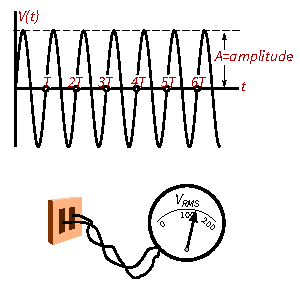
\includegraphics{01RMSvoltage.pdf}

The 110 Volts that is specified is not the amplitude $A$ of the oscillation, but
instead it refers to the ``\textit{Root Mean Square}'' of the voltage.
By definition the R.M.S.~of the oscillating voltage $V(t)$ is
\[
110 = \sqrt{\frac{1}{T}\int_0^T V(t)^2 \dd t}.
\]
(it is the square root of the mean of the square of $V(t)$).

Compute the amplitude $A$.


\end{multicols}

\noproblemfont

\section{Integration by Parts}\label{sec:integration-by-parts} %{{{1
While the double angle trick is just that, a (useful) trick, the method of
\emph{integration by parts} is very general and appears in many different forms.
It is the integration counterpart of the product rule for differentiation.

\subsection{The product rule and integration by parts} %{{{2
Recall that the product rule says that
\[
\frac{\dd F(x)G(x)}{\dd x}=\frac{\dd F(x)}{\dd x}G(x)+F(x)\frac{\dd G(x)}{\dd x}
\]
and therefore, after rearranging terms,
\[
F(x)\frac{\dd G(x)}{\dd x} = \frac{\dd F(x)G(x)}{\dd x} - \frac{\dd F(x)}{\dd
  x}G(x) .
\]
If we integrate both sides we get the formula for \emph{integration by parts}
\[
\int F(x)\frac{\dd G(x)}{\dd x}\,\dd x=F(x)G(x)-\int \frac{\dd F(x)}{\dd
  x}G(x)\,\dd x.
\]
Note that the effect of integration by parts is to integrate one part of the
function ($G'(x)$ got replaced by $G(x)$) and to differentiate the other part
($F(x)$ got replaced by $F'(x)$).  For any given integral there are many ways of
choosing $F$ and $G$, and it not always easy to see what the best choice is.


\subsection{An Example -- Integrating by parts once} %{{{2
Consider the problem of finding
\[
I = \int xe^x \; \dd x.
\]
We can use integration by parts as follows:
\[
\int \underbrace{x}_{F(x)}\underbrace{e^{x}}_{G'(x)}\,\dd x
=\underbrace{x}_{F(x)}\underbrace{e^{x}}_{G(x)} -\int
\underbrace{e^{x}}_{G(x)}\underbrace1_{F'(x)}\,\dd x = xe^x-e^x +C.
\]
Observe that in this example $e^x$ was easy to integrate, while the factor $x$
becomes an easier function when you differentiate it.  This is the usual state
of affairs when integration by parts works: differentiating one of the factors
($F(x)$) should simplify the integral, while integrating the other ($G'(x)$)
should not complicate things (too much).

\subsection{Another example} What is %{{{2
\[
\int x\sin x\;\dd x ?
\]
Since $\sin x = \frac{\dd (-\cos x)}{\dd x}$ we can integrate by parts
\[
\int \underbrace{x}_{F(x)}\underbrace{\sin x}_{G'(x)}\,\dd x
=\underbrace{x}_{F(x)} \underbrace{(-\cos x)}_{G(x)} - \int
\underbrace{1}_{F'(x)}\cdot\underbrace{(-\cos x)}_{G(x)}\,\dd x =-x\cos x+\sin
x+C.
\]

\subsection{Example -- Repeated Integration by Parts} %{{{2
Let's try to compute
\[
I = \int x^2 e^{2x}\;\dd x
\]
by integrating by parts.  Since $e^{2x}=\frac{\dd\frac12e^{2x} }{\dd x}$ one has
\begin{equation}
  \int \underbrace{x^{2}}_{F(x)}\underbrace{e^{2x}}_{G'(x)}\,\dd x
  =  x^{2}\frac{e^{2x}}{2}-\int \frac{e^{2x}}{2}2x\,\dd x
  =  \frac12x^{2}e^{2x}-\int e^{2x}x\,\dd x.
  \label{eq:01integration-by-parts-1}
\end{equation}
To do the integral on the left we have to integrate by parts again:
\[
\int e^{2x}x\,\dd x = \underbrace{\frac12 e^{2x}}_{G(x)} \underbrace{x}_{F(x)} -
\int \underbrace{\frac12 e^{2x}}_{G(x)} \underbrace{1}_{F'(x)}\,\dd x.  =
\frac12 xe^{2x} - \frac12 \int e^{2x}\,\dd x = \frac12 xe^{2x} - \frac14 e^{2x}
+C.
\]
Combining this with \eqref{eq:01integration-by-parts-1} we get
\[
\int x^2 e^{2x}\;\dd x =
\frac{1}{2}x^{2}e^{2x}-\frac{1}{2}xe^{2x}+\frac{1}{4}e^{2x}-C
\]
(Be careful with all the minus signs that appear when integrating by parts.)

\subsection{Another example of repeated integration by parts} The same procedure %{{{2
as in the previous example will work whenever we have to integrate
\[
\int P(x)e^{ax}\,\dd x
\]
where \( P(x) \) is any polynomial, and \( a \) is a constant.  Every time we
integrate by parts, we get this
\begin{align*}
  \int \underbrace{P(x)}_{F(x)}\underbrace{e^{ax}}_{G'(x)}\,\dd x
  & =  P(x)\frac{e^{ax}}{a}-\int \frac{e^{ax}}{a}P'(x)\,\dd x\\
  & = \frac{1}{a}P(x)e^{ax}-\frac{1}{a}\int P'(x)e^{ax}\,\dd x.
\end{align*}
We have replaced the integral \( \int P(x)e^{ax}\,\dd x \) with the integral \(
\int P'(x)e^{ax}\,\dd x \). This is the same kind of integral, but it is a
little easier since the degree of the derivative \( P'(x) \) is less than the
degree of \( P(x) \).

\subsection{Example -- sometimes the factor $G'(x)$ is invisible} %{{{2
Here is how we can get the antiderivative of $\ln x$ by integrating by parts:
\begin{align*}
  \int \ln x\,\dd x
  &= \int \underbrace{\ln x}_{F(x)}\cdot \underbrace{1}_{G'(x)}\,\dd x \\
  &= \ln x\cdot x - \int \frac1x\cdot x\,\dd x \\
  &= x\ln x - \int 1\,\dd x \\
  &= x\ln x -x + C.
\end{align*}
We can do $\int P(x)\ln x\,\dd x$ in the same way if $P(x)$ is any polynomial.
For instance, to compute
\[
\int (z^2+z) \ln z \,\dd z
\]
we integrate by parts:
\begin{align*}
  \int \underbrace{(z^2+z)}_{G'(z)} \underbrace{\ln z}_{F(z)} \,\dd z &=
  \bigl(\tfrac13 z^3 + \tfrac 12 z^2\bigr) \ln z
  - \int  \bigl(\tfrac13 z^3 + \tfrac 12 z^2\bigr) \frac 1 z\, \dd z \\
  &= \bigl(\tfrac13 z^3 + \tfrac 12 z^2\bigr) \ln z
  - \int  \bigl(\tfrac13 z^2 + \tfrac 12 z\bigr)\, \dd z \\
  &= \bigl(\tfrac13 z^3 + \tfrac 12 z^2\bigr) \ln z -\tfrac19 z^3 - \tfrac 14
  z^2 +C.
\end{align*}

\subsection{An example where we get the original integral back} %{{{2
It can happen that after integrating by parts a few times the integral we get is
the same as the one we started with.  When this happens we have found an
equation for the integral, which we can then try to solve.  The standard example
in which this happens is the integral
\[
I = \int e^x \sin 2x\, \dd x.
\]
We integrate by parts twice:
\begin{align*}
  \int \underbrace{e^x}_{F'(x)} \underbrace{\sin 2x}_{G(x)}\, \dd x
  & = e^x \sin 2x - \int \underbrace{e^x}_{F(x)} \underbrace{2\cos 2x}_{G'(x)} \, \dd x \\
  &=  e^x \sin 2x - 2 \int e^x \cos 2x \, \dd x \\
  &=  e^x \sin 2x - 2 e^x \cos 2x - 2\int e^x 2\sin 2x\, \dd x \\
  &= e^x \sin 2x - 2 e^x \cos 2x - 4\int e^x \sin 2x\, \dd x .
\end{align*}
Note that the last integral here is exactly $I$ again.  Therefore the integral
$I$ satisfies
\[
I = e^x \sin 2x - 2 e^x \cos 2x - 4I.
\]
We solve this equation for $I$, with result
\[
5I = e^x \sin 2x - 2 e^x \cos 2x \implies I = \frac15\bigl( e^x \sin 2x - 2 e^x
\cos 2x\bigr).
\]
Since $I$ is an indefinite integral we still have to add the arbitrary constant:
\[
I = \frac15\bigl( e^x \sin 2x - 2 e^x \cos 2x\bigr) + C.
\]

\section{Reduction Formulas}\label{sec:reduction-formulas} %{{{1
We have seen that we can compute integrals by integrating by parts, and that we
sometimes have to integrate by parts more than once to get the answer.  There
are integrals where we have to integrate by parts not once, not twice, but
$n$-times before the answer shows up.  To do such integrals it is useful to
carefully describe what happens each time we integrate by parts before we do the
actual integrations.  The formula that describes what happens after one partial
integration is called a \emph{reduction formula.}  All this is best explained by
an example.


\subsection{First example of a reduction formula} Consider the integral %{{{2
\[
I_n = \int x^n e^{ax}\,\dd x, \qquad (n=0,1,2,3,\ldots)
\]
or, in other words, consider all the integrals
\[
I_0 = \int e^{ax}\,\dd x, \quad I_1 = \int xe^{ax}\, \dd x, \quad I_2 = \int
x^2e^{ax}\, \dd x, \quad I_3 = \int x^3e^{ax}\, \dd x, \ldots
\]
and so on.  We will consider all these integrals at the same time.

Integration by parts in $I_n$ gives us
\begin{align*}
  I_n &= \int \underbrace{x^n}_{F(x)} \underbrace{e^{ax}}_{G'(x)} \,\dd x\\
  &= x^n\frac1ae^{ax} -\int nx^{n-1}\frac1a e^{ax}\,\dd x \\
  &= \frac 1a x^n e^{ax} - \frac na \int x^{n-1}e^{ax}\,\dd x.
\end{align*}
We haven't computed the integral, and in fact the integral that we still have to
do is of the same kind as the one we started with (integral of $x^{n-1}e^{ax}$
instead of $x^ne^{ax}$). What we have derived is the following \emph{reduction
  formula}
\[
I_n = \frac 1a x^n e^{ax} - \frac na I_{n-1},
\]
which holds for all $n$.

For $n=0$ we do not need the reduction formula to find the integral.  We have
\[
I_0 = \int e^{ax}\,\dd x = \frac{1} {a} e^{ax} +C.
\]
When $n\neq0$ the reduction formula tells us that we have to compute $I_{n-1}$
if we want to find $I_n$. The point of a reduction formula is that the same
formula also applies to $I_{n-1}$, and $I_{n-2}$, etc., so that after repeated
application of the formula we end up with $I_0$, i.e., an integral we know.

For example, if we want to compute $\int x^3 e^{ax}\,\dd x$ we use the reduction
formula three times:
\begin{align*}
  I_3
  &= \frac 1a x^3 e^{ax} - \frac 3a I_2 \\
  &=\frac 1a x^3 e^{ax}
  - \frac 3a \left\{\frac 1a x^2 e^{ax} - \frac 2a I_1\right\} \\
  &=\frac 1a x^3 e^{ax} - \frac 3a \left\{\frac 1a x^2 e^{ax} - \frac 2a
    \left(\frac 1a x e^{ax} - \frac 1a I_0 \right)\right\}
\end{align*}
Insert the known integral $I_0= \frac1a e^{ax} +C$ and simplify the other terms
and we get
\[
\int x^3e^{ax}\,\dd x = \frac 1a x^3 e^{ax} -\frac 3{a^2} x^2 e^{ax} +\frac
6{a^3} x e^{ax} -\frac 6{a^4} e^{ax}+C.
\]


\subsection{Reduction formula requiring two partial integrations} %{{{2
Consider
\[
S_n = \int x^n \sin x\,\dd x.
\]
Then for $n\geq 2$ one has
\begin{align*}
  S_n
  &= -x^n\cos x +n\int x^{n-1}\cos x\,\dd x \\
  &= -x^n\cos x +n x^{n-1}\sin x - n (n-1)\int x^{n-2}\sin x\,\dd x.
\end{align*}
Thus we find the reduction formula
\[
S_n = -x^n\cos x +n x^{n-1}\sin x - n (n-1)S_{n-2}.
\]
Each time we use this reduction, the exponent $n$ drops by 2, so in the end we
get either $S_1$ or $S_0$, depending on whether we started with an odd or even
$n$.  These two integrals are
\begin{align*}
  S_0 &= \int \sin x\,\dd x = -\cos x + C \\
  S_1 &= \int x\sin x\, \dd x = -x\cos x+\sin x +C.
\end{align*}
(Integrate by parts once to find $S_1$.)

As an example of how to use the reduction formulas for $S_n$ let's try to
compute $S_4$:
\begin{align*}
  \int x^4\sin x \, \dd x
  &= S_4 = -x^4 \cos x + 4x^3 \sin x - 4\cdot 3 S_2 \\
  &= -x^4 \cos x + 4x^3 \sin x - 4\cdot 3 \cdot \bigl\{-x^2\cos x +2x\sin x -
  2\cdot1 S_0\bigr\}
\end{align*}
At this point we use $S_0 = \int \sin x\, \dd x = -\cos x+C$, and we combine
like terms.  This results in
\begin{align*}
  \int x^4\sin x \, \dd x\
  &= -x^4 \cos x + 4x^3 \sin x \\
  & \qquad \qquad- 4\cdot 3 \cdot \bigl\{-x^2\cos x +2x\sin x - 2\cdot1 (-\cos x)\bigr\} + C\\
  & = \bigl(-x^4 +12x^2-24\bigr) \cos x + \bigl(4x^3+24x \bigr)\sin x +C.
\end{align*}

\subsection{A reduction formula where you have to solve for $I_n$} %{{{2
\label{sec:01sin-n-x-reduction-formula}
We try to compute
\[
I_n = \int (\sin x)^n\,\dd x
\]
by a reduction formula. Integrating by parts we get
\begin{align*}
  I_n
  &= \int (\sin x)^{n-1}\sin x\,\dd x \\
  &= - (\sin x)^{n-1}\cos x
  -\int (-\cos x) (n-1) (\sin x)^{n-2}\cos x\,\dd x \\
  &= - (\sin x)^{n-1}\cos x +(n-1)\int (\sin x)^{n-2} \cos^2x\,\dd x.
\end{align*}
We now use $\cos^2x=1-\sin^2x$, which gives
\begin{align*}
  I_n &= - (\sin x)^{n-1}\cos x
  +(n-1)\int\left\{\sin^{n-2}x-\sin^n x\right\}\,\dd x \\
  &= - (\sin x)^{n-1}\cos x + (n-1)I_{n-2}- (n-1)I_n.
\end{align*}
We can think of this as an equation for $I_n$, which, when we solve it tells us
\[
nI_n = - (\sin x)^{n-1}\cos x + (n-1)I_{n-2}
\]
and thus implies
\begin{equation}
  I_n = -\frac1n \sin^{n-1}x\cos x + \frac{n-1}n I_{n-2}.
  \label{eq:01reduction-formula-sinx-n}
\end{equation}
Since we know the integrals
\begin{align*}
  I_0&= \int (\sin x)^0\dd x = \int\dd x = x+C\\
  \intertext{and} I_1&= \int \sin x\,\dd x = -\cos x+C
\end{align*}
the reduction formula \eqref{eq:01reduction-formula-sinx-n} allows us to
calculate $I_n$ for any $n\geq2$.


\subsection{A reduction formula that will come in handy later} %{{{2
\label{sec:01pt-fracs-reduction}
In the next section we will see how the integral of any ``rational function''
can be transformed into integrals of easier functions, the most difficult of
which turns out to be
\[
I_n = \int \frac{\dd x}{(1+x^2)^n}.
\]
When $n=1$ this is a standard integral, namely
\[
I_1 = \int\frac{\dd x}{1+x^2} = \arctan x +C.
\]
When $n>1$ integration by parts gives us a reduction formula.  Here's the
computation:
\begin{align*}
  I_n &=  \int (1+x^2)^{-n}\,\dd x \\
  &=  \frac{ x}{(1+x^2)^n} - \int x\, (-n)\bigl(1+x^2\bigr)^{-n-1}\,2x\,\dd x \\
  &= \frac{ x}{(1+x^2)^n} +2n\int \frac{x^2} {(1+x^2)^{n+1}}\,\dd x
\end{align*}
Apply
\[
\dfrac{x^2} {(1+x^2)^{n+1}} =\dfrac{(1+x^2) -1} {(1+x^2)^{n+1}} = \frac{1}
{(1+x^2)^{n}}-\frac{1} {(1+x^2)^{n+1}}
\]
to get
\[
\int \frac{x^2} {(1+x^2)^{n+1}}\,\dd x =\int\left\{ \frac{1}
  {(1+x^2)^{n}}-\frac{1} {(1+x^2)^{n+1}}\right\}\,\dd x =I_n - I_{n+1}.
\]
Our integration by parts therefore told us that
\[
I_n = \frac{ x}{(1+x^2)^n} +2n\bigl(I_n-I_{n+1}\bigr),
\]
which we can solve for $I_{n+1}$. We find the reduction formula
\[
I_{n+1} = \frac1{2n}\frac{x}{(1+x^2)^n}+\frac{2n-1}{2n} I_n.
\]

As an example of how we can use it, we start with $I_1=\arctan x+C$, and
conclude that
\begin{align*}
  \int\frac{\dd x}{(1+x^2)^2}
  &= I_2 =I_{1+1} \\
  &=\frac1{2\cdot1}\frac{x}{(1+x^2)^1}+\frac{2\cdot1-1}{2\cdot1} I_1 \\
  &= \tfrac12\frac{x}{1+x^2}+\tfrac12 \arctan x +C.
\end{align*}
Apply the reduction formula again, now with $n=2$, and we get
\begin{align*}
  \int\frac{\dd x}{(1+x^2)^3} &= I_3 = I_{2+1} \\
  &= \frac1{2\cdot2}\frac{x}{(1+x^2)^2}+\frac{2\cdot2-1}{2\cdot2} I_2 \\
  &= \tfrac14\frac{x}{(1+x^2)^2}+\tfrac{3}{4} \left\{
    \tfrac12\frac{x}{1+x^2}+\tfrac{1}{2} \arctan x
  \right\} \\
  &= \tfrac14\frac{x}{(1+x^2)^2} +\tfrac{3}{8}\frac{x}{1+x^2} +\tfrac{3}{8}
  \arctan x +C.
\end{align*}

\section{Problems} %{{{1
\label{sec:integration-by-parts-problems}
\problemfont %{{{3
\begin{multicols}{2}
\problem Evaluate $\DS \int x^n \ln x\,\dd x$ where $n\ne-1$. %{{{3
\answer %{{{3
$\DS \int x^n \ln x\,\dd x
= \frac{x^{n+1}\ln x}{n+1} - \frac{x^{n+1}}{(n+1)^2}+C$.
\endanswer

\problem\label{pblm:integral-eax-sinbx} Assume $a$ and $b$ are constants, and %{{{3
compute $\DS \int e^{ax}\sin bx\,\dd x$.  [Hint: Integrate by parts twice; you
can assume that $b\neq0$.]
\answer %{{{3
$\DS\int e^{ax}\sin bx\,\dd x= \frac{e^{ax}}{a^2+b^2}(a\sin bx
-b\cos bx)+C.$
\endanswer

\problem Evaluate $\DS\int e^{ax}\cos bx\,\dd x$ where $a, b\ne 0$. %{{{3
\answer %{{{3
$\DS\int e^{ax}\cos bx\,\dd x
= \frac{e^{ax}}{a^2+b^2}(a\cos bx+b\sin bx)+C.$
\endanswer



\problem Prove the formula %{{{3
\[
\int x^n e^x\,\dd x= x^ne^x-n\int x^{n-1}e^x\,\dd x
\]
and use it to evaluate $\DS\int x^2e^x\,\dd x$.

\problem Use \S\ref{sec:01sin-n-x-reduction-formula} to evaluate %{{{3
$\DS\int\sin^2x\,\dd x$.  Show that the answer is the same as the answer you get
using the half angle formula.

\problem Use the reduction formula in \S\ref{sec:01sin-n-x-reduction-formula} to %{{{3
compute $\DS \int_0^{\pi/2} \sin^{14}x \dd x$.
\answer %{{{3
$\int_0^{\pi} \sin^{14}x \dd x = \frac{13\cdot11\cdot9\cdot7\cdot5\cdot3\cdot1 }
{14\cdot12\cdot10\cdot8\cdot6\cdot4\cdot2}\frac{\pi}{2}$
\endanswer

\problem In this problem you'll look at the numbers  %{{{3
\[
A_n = \int_0^\pi \sin^n x \, \dd x.
\]
\subprob Check that $A_0 = \pi$ and $A_1 = 2$.

\subprob
Use the reduction formula in \S\ref{sec:01sin-n-x-reduction-formula} to
compute  $A_5$, $A_6$, and $A_7$.
\answer %{{{3
$\int_0^\pi \sin^5x \dd x = \frac{4\cdot2}{5\cdot3}\cdot2$\\
$\int_0^{\pi} \sin^{6}x \dd x = \frac{5\cdot3\cdot1 }
{6\cdot4\cdot2}\pi$\\
$\int_0^\pi \sin^7x \dd x = \frac{6\cdot4\cdot2}{7\cdot5\cdot3}\cdot2$
\endanswer

\subprob  Explain why
\[
A_n < A_{n-1} 
\]
is true for all $n=1, 2, 3, 4, \ldots$

(Hint: Interpret the integrals $A_n$ as area under the graph, and check that
$(\sin x)^n \leq (\sin x)^{n-1}$ for all $x$.)

\subprob $\carefulnow$ Based on your values for $A_5$, $A_6$, and $A_7$ find two
fractions $a$ and $b$ such that $a<\pi<b$.

\problem Prove the formula %{{{3
\begin{multline*}
  \int \cos^nx\,\dd x
  = \\
  \frac1n{\sin x\cos^{n-1}x} \\
  +\frac{n-1}{n}\int\cos^{n-2}x\,\dd x,
\end{multline*}
for $n\neq0$, and use it to evaluate
\[
\int_0^{\pi/4}\cos^4x\,\dd x.
\]
\answer %{{{3
$\int \cos^n x \dd x = \frac1n\sin x \cos^{n-1}x
+\frac{n-1}n\int\cos^{n-2}x \dd x$;
\[
  \int \cos^4 x\,\dd x = 
  \frac38 x+ \frac14 \cos^3x\,\sin x + \frac38\cos x\,\sin x +C
\]
Setting $x=0$ and $x=\pi/4$ leads to
$\int_0^{\pi/4}\cos^4 x \dd x = \frac14+ \frac3{32}\pi$
\endanswer

\problem Prove the formula %{{{3
\begin{multline*}
  \int x^m(\ln x)^n\,\dd x=\\
  \frac{x^{m+1}(\ln x)^n}{m+1} \\
  - \frac{n}{m+1}\int x^m(\ln x)^{n-1}\,\dd x,
\end{multline*}
for $m\neq -1$, and use it to evaluate the following integrals:
\answer %{{{3
Hint: first integrate $x^m$.
\endanswer
\problem $\DS\int \ln x\,\dd x$ %{{{3
\answer %{{{3
$x\ln x-x+C$
\endanswer
\problem $\DS\int (\ln x)^2\,\dd x$ %{{{3
\answer %{{{3
$x(\ln x)^2-2x\ln x+2x+C$
\endanswer
\problem $\DS\int x^3(\ln x)^2\,\dd x$ %{{{3
\problem Evaluate $\DS\int x^{-1}\ln x\,\dd x$ by another %{{{3
method. [Hint: the solution is short!]
\answer %{{{3
Substitute $u=\ln x$.
\endanswer

\problem For any integer $n > 1$ derive the formula %{{{3
\[
\int \tan^n x\,\dd x=\frac{\tan^{n-1}x}{n-1}-\int \tan^{n-2}x\,\dd x
\]
Using this, find $\DS\int_0^{\pi/4} \tan^5x\,\dd x$.
\answer %{{{3
$\int_0^{\pi/4}\tan^5 x\dd x =
\frac14(1)^4-\frac12(1)^2 + \int_0^{\pi/4}\tan x \dd x =
-\frac14+\ln\frac12\surd2$
\endanswer

\noindent%
Use the reduction formula from example~\ref{sec:01pt-fracs-reduction} to compute
these integrals:
\problem $\DS \int \frac{\dd x}{(1+x^2)^3}$ %{{{3

\problem $\DS \int \frac{\dd x}{(1+x^2)^4}$ %{{{3

\problem $\DS \int \frac{x\dd x}{(1+x^2)^4}$ %{{{3
[Hint: $\int x/ (1+x^2)^n \dd x$ is easy.]
\answer %{{{3
Substitute $u=1+x^2$.
\endanswer

\problem $\DS \int \frac{1+ x}{(1+x^2)^2}\,\dd x$ %{{{3

\problem $\DS \int\frac{\dd x}{\bigl(49+x^2\bigr)^3}$. %{{{3

\problem The reduction formula from example~\ref{sec:01pt-fracs-reduction} is %{{{3
valid for all $n\neq0$. In particular, $n$ does not have to be an integer, and
it does not have to be positive.  Find a relation between $\DS\int
\sqrt{1+x^2}\,\dd x$ and $\DS\int\frac{\dd x}{\sqrt{1+x^2}}$ by setting
$n=-\frac12$.

\problem Apply integration by parts to %{{{3
\[
\int \frac1x \;\dd x
\]
Let
$u=\frac1x$ and $dv=\dd x$.  This gives us,\ $\dd u=\frac{-1}{\;x^2}\,\dd x$
and $v=x$.
\[\int \frac1x \;\dd x = (\frac1x)(x) -\int x\;\frac{-1}{\;x^2}\;\dd x\]
Simplifying
\[\int \frac1x \;\dd x = 1 + \int \frac1x \;\dd x\]
and subtracting the integral from both sides gives us $0=1$.
How can this be?

\end{multicols}
\noproblemfont

\section{Partial Fraction Expansion} %{{{1
\label{sec:partial-fractions}
By definition, a \emph{rational function} is a quotient (a \textit{ratio}) of
polynomials,
\[
f(x) = \frac{P(x)}{Q(x)} = \frac{p_nx^n+p_{n-1}x^{n-1}+\cdots+p_1x+p_0}
{q_dx^d+q_{d-1}x^{d-1}+\cdots+q_1x+q_0}.
\]
Such rational functions can always be integrated, and the trick that allows you
to do this is called a \emph{partial fraction expansion}.  The whole procedure
consists of several steps that are explained in this section.  The procedure
itself has nothing to do with integration: it's just a way of rewriting rational
functions.  It is in fact useful in other situations, such as finding Taylor
expansions (see Chapter~\ref{cha:taylor}) and computing ``inverse Laplace
transforms'' (see \textsc{Math} 319.)


\subsection{Reduce to a proper rational function} %{{{2
\label{sec:reduce-prop-rati}
A \emph{proper rational function} is a rational function $P(x)/Q (x)$ where the
degree of $P(x)$ is strictly less than the degree of $Q(x)$.  The method of
partial fractions only applies to proper rational functions.  Fortunately
there's an additional trick for dealing with rational functions that are not
proper.

If $P/Q$ isn't proper, i.e.\ if $\mathrm{degree}(P)\geq\mathrm{degree} (Q)$,
then you divide $P$ by $Q$, with result
\[
\frac{P(x)}{Q(x)} = S(x)+ \frac{R(x)}{Q(x)}
\]
where $S (x)$ is the quotient, and $R (x)$ is the remainder after division. In
practice you would do a long division to find $S(x)$ and $R(x)$.


\subsection{Example} Consider the rational function %{{{2
\[
f (x) = \frac{x^3-2x+2}{x^2-1}.
\]
Here the numerator has degree 3 which is more than the degree of the denominator
(which is 2).  The function $f(x)$ is therefore not a proper rational function.
To apply the method of partial fractions we must first do a division with
remainder. One has
\begin{center}
  \begin{tabular} {c*{6}{@{}r}} % @{#!}*&#@ who came up with this #@!% notation?
    & &$x$ & & && $=S(x)$ \\ \cline{3-6}
    $x^2-1$ &\; \rule[-3pt]{1pt}{15pt}& $x^3$ &  & $-2x$ & $+2$& \\
    && \;$x^3$ &  & $-x$ & & \\ \cline{3-6}
    &  &&     & $-x$ & $+2$ & \ $=R(x)$ \rule{0pt}{12pt}\\
  \end{tabular}
\end{center}
so that
\[
f (x) = \frac{x^3-2x+2}{x^2-1} = x + \frac{-x+2}{x^2-1}
\]
When we integrate we get
\begin{align*}
  \int \frac{x^3-2x+2}{x^2-1}\,\dd x
  &=\int\left\{x+ \frac{-x+2}{x^2-1}\right\}\,\dd x\\
  &=\frac{x^2}{2} +\int \frac{-x+2}{x^2-1}\,\dd x.
\end{align*}
The rational function that we still have to integrate, namely
$\frac{-x+2}{x^2-1}$, is proper: its numerator has lower degree than its
denominator.



\subsection{Partial Fraction Expansion: The Easy Case} %{{{2
To compute the partial fraction expansion of a proper rational function
$P(x)/Q(x)$ you must factor the denominator $Q(x)$.  Factoring the denominator
is a problem as difficult as finding all of its roots; in Math~222 we shall only
do problems where the denominator is already factored into linear and quadratic
factors, or where this factorization is easy to find.

In the easiest partial fractions problems, all the roots of $Q(x)$ are real
numbers and distinct, so the denominator is factored into distinct linear
factors, say
\[
\frac{P(x)}{Q(x)} = \frac{P(x)}{(x-a_1)(x-a_2)\cdots(x-a_n)}.
\]
To integrate this function we find constants $A_1,A_2,\ldots,A_n$ so that
\[
\frac{P(x)}{Q(x)} = \frac{A_1}{x-a_1} + \frac{A_2}{x-a_2}+\cdots+
\frac{A_n}{x-a_n}.  \eqno(\#)
\]
Then the integral is
\[
\int \frac{P(x)}{Q(x)}\,\dd x =
A_1\ln|x-a_1|+A_2\ln|x-a_2|+\cdots+A_n\ln|x-a_n|+C.
\]


One way to find the coefficients $A_i$ in~$(\#)$ is called the \emph{method of
  equating coefficients}.  In this method we multiply both sides of~(\#) with
$Q(x) = (x-a_1)\cdots (x-a_n)$. The result is a polynomial of degree $n$ on both
sides. Equating the coefficients of these polynomial gives a system of $n$
linear equations for $A_1$, \ldots, $A_n$. You get the $A_i$ by solving that
system of equations.

Another much faster way to find the coefficients $A_i$ is the \emph{Heaviside
  trick}\footnote{~Named after \textsc{Oliver Heaviside}, a physicist and
  electrical engineer in the late 19$^{\mathrm{th}}$ and early
  20$^{\mathrm{th}}$ century.}.  Multiply equation~$(\#)$ by $x-a_i$ and then
plug in\footnote{~More properly, you should take the limit $x\to a_i$.  The
  problem here is that equation~$(\#)$ has $x-a_i$ in the denominator, so that
  it does not hold for $x=a_i$.  Therefore you cannot set $x$ equal to $a_i$ in
  any equation derived from~$(\#)$.  But you can take the limit $x\to a_i$,
  which in practice is just as good.}  $x=a_i$.  On the right you are left with
$A_i$ so
\[
A_i=\left.\frac{P(x)(x-a_i)}{Q(x)}\right|_{x=a_i}=
\frac{P(a_i)}{(a_i-a_1)\cdots(a_i-a_{i-1})(a_i-a_{i+1})\cdots(a_i-a_n)}.
\]
\subsection{Previous Example continued} %{{{2
To integrate $\dfrac{-x+2}{x^2-1}$ we factor the denominator,
\[
x^2 -1 = (x-1) (x+1).
\]
The partial fraction expansion of $\dfrac{-x+2}{x^2-1}$ then is
\begin{equation}
  \frac{-x+2}{x^2-1} =\frac{-x+2}{(x-1) (x+1)} =\frac A{x-1} + \frac B{x+1}.
  \label{eq:01partial-fractions-1}
\end{equation}
Multiply with $(x-1) (x+1)$ to get
\[
-x+2 = A (x+1)+B (x-1) = (A+B) x + (A-B).
\]
The functions of $x$ on the left and right are equal only if the coefficient of
$x$ and the constant term are equal. In other words we must have
\[
A+B = -1 \quad\text{ and }\quad A-B=2.
\]
These are two linear equations for two unknowns $A$ and $B$, which we now
proceed to solve.  Adding both equations gives $2A=1$, so that $A=\frac12$; from
the first equation one then finds $B=-1-A=-\frac32$. So
\[
\frac{-x+2}{x^2-1} = \frac{1/2}{x-1}-\frac{3/2}{x+1}.
\]
Instead, we could also use the Heaviside trick:
multiply~\eqref{eq:01partial-fractions-1} with $x-1$ to get
\[
\frac{-x+2}{x+1} = A+B\frac{x-1}{x+1}
\]
Take the limit $x\to1$ and you find
\[
\frac{-1+2}{1+1}=A, \text{ i.e. } A=\frac12.
\]
Similarly, after multiplying~\eqref{eq:01partial-fractions-1} with $x+1$ one
gets
\[
\frac{-x+2}{x-1}=A\frac{x+1}{x-1} + B,
\]
and letting $x\to-1$ you find
\[
B= \frac{- (-1)+2}{(-1)-1} = -\frac 32,
\]
as before.

Either way, the integral is now easily found, namely,
\begin{align*}
  \int \frac{x^3-2x+1}{x^2-1}\,\dd x
  &=\frac{x^2}{2} +\int  \frac{-x+2}{x^2-1}\,\dd x \\
  &= \frac{x^2}2+\int\left\{\frac{1/2}{x-1}-\frac{3/2}{x+1}\right\}\,\dd x\\
  &=\frac{x^2}2+\frac12\ln|x-1|-\frac32\ln|x+1|+C.
\end{align*}



\subsection{Partial Fraction Expansion: The General Case} %{{{2
When the denominator $Q(x)$ contains repeated factors or quadratic factors (or
both) the partial fraction decomposition is more complicated.  In the most
general case the denominator $Q(x)$ can be factored in the form
\begin{equation}\label{eq:Q-yuck}
  Q(x)=(x-a_1)^{k_1}\cdots(x-a_n)^{k_n}(x^2+b_1x+c_1)^{\ell_1}\cdots(x^2+b_mx+c_m)^{\ell_m}
\end{equation}
Here we assume that the factors $x-a_1$, \ldots, $x-a_n$ are all different, and
we also assume that the factors $x^2+b_1x+c_1 $, \ldots, $ x^2+b_mx+c_m$ are all
different.

It is a theorem from advanced algebra that you can always write the rational
function $P(x)/Q(x)$ as a sum of terms like this
\begin{equation}
  \label{eq:yuck-decomposed}
  \frac{P(x)}{Q(x)} =
  \cdots+\frac{A}{(x-a_i)^k}+\cdots+\frac{Bx+C}{(x^2+b_jx+c_j)^\ell}+\cdots
\end{equation}

How did this sum come about?

For each linear factor $(x-a)^{k}$ in the denominator (\ref{eq:Q-yuck}) you get
terms
\[
\frac{A_1}{x-a}+\frac{A_2}{(x-a)^2}+\cdots+\frac{A_k}{(x-a)^k}
\]
in the decomposition. There are as many terms as the exponent of the linear
factor that generated them.

For each quadratic factor $(x^2+bx+c)^\ell$ you get terms
\[
\frac{B_1x+C_1}{x^2+bx+c}+\frac{B_2x+C_2}{(x^2+bx+c)^2}+\cdots
+\frac{B_mx+C_m}{(x^2+bx+c)^\ell}.
\]
Again, there are as many terms as the exponent $\ell$ with which the quadratic
factor appears in the denominator (\ref{eq:Q-yuck}).

In general, you find the constants $A_{\ldots}$, $B_{\ldots}$ and $C_{\ldots}$
by the method of equating coefficients.

\medskip\noindent {\Large \textdbend }\hfill\parbox[b]{4in}{\itshape
  Unfortunately, in the presence of quadratic factors or repeated linear factors
  the Heaviside trick does not give the whole answer; we really have to use the
  method of equating coefficients.}\hfill{\Large \textdbend } \medskip

The workings of this method are best explained in an example.

\subsection{Example} %{{{2
Find the partial fraction decomposition of
\[
f(x) = \frac{x^2+2} {x^2(x^2+1)}
\]
and compute
\[
I = \int \frac{x^2+2} {x^2(x^2+1)} \, \dd x.
\]
The degree of the denominator $x^2(x^2+1)$ is four, so our partial fraction
decomposition must also contain four undetermined constants.  The expansion
should be of the form
\[
\frac{x^2+2} {\color{blue}x^2\color{badgerred}(x^2+1)} = \color{blue}\frac{A}
{x} +\frac{B} {x^2} \color{black}+ \color{badgerred} \frac{Cx+D} {x^2+1}.
\]
To find the coefficients $A,B,C,D$ we multiply both sides with $x^2(1+x^2)$,
\begin{align*}
  x^2+2 &= A x(x^2+1) + B(x^2+1) + x^2(Cx+D)\\
  x^2+2 &= (A+C)x^3 + (B+D)x^2 + Ax + B \\
  0\cdot x^3+ 1\cdot x^2+0\cdot x+2 &= (A+C)x^3 + (B+D)x^2 + Ax + B
\end{align*}
Comparing terms with the same power of $x$ we find that
\[
A+C = 0, \quad B+D = 1, \quad A = 0, \quad B=2.
\]
These are four equations for four unknowns.  Fortunately for us they are not
very difficult in this example.  We find $A=0$, $B=2$, $C=-A=0$, and $D=1-B =
-1$, whence
\[
f(x) = \frac{x^2+2} {x^2(x^2+1)} = \frac{2} {x^2} - \frac{1} {x^2+1}.
\]
The integral is therefore
\[
I = \frac{x^2+2} {x^2(x^2+1)} \,\dd x =-\frac{2} {x} - \arctan x +C.
\]
\subsection{A complicated example} %{{{2
Find the integral
\[
\int\frac{x^2+3}{x^2(x+1)(x^2+1)^3}\,\dd x.
\]
The procedure is exactly the same as in the previous example.  We have to expand
the integrand in partial fractions:
\begin{multline}
  \frac{x^2+3}{\color{blue}x^2\color{badgerred}(x+1)\color{darkgreen}(x^2+1)^3}
  = \color{blue}\frac{A_1}{x}+ \frac{A_2}{x^2}+\color{badgerred}\frac{A_3}{x+1}\\
  +\color{darkgreen} \frac{B_1x+C_1}{x^2+1} +\frac{B_2x+C_2}{(x^2+1)^2}
  +\frac{B_3x+C_3}{(x^2+1)^3}.
  \label{eq:01partial-fraction-example}
\end{multline}
Note that the degree of the denominator $x^2(x+1)(x^2+1)^3$ is $2+1+3\times2 =
9$, and also that the partial fraction decomposition has nine undetermined
constants $A_1$, $A_2$, $A_3$, $B_1$, $C_1$, $B_2$, $C_2$, $ B_3$, $C_3$.  After
multiplying both sides of \eqref{eq:01partial-fraction-example} with the
denominator $x^2(x+1)(x^2+1)^3$, expanding everything, and then equating
coefficients of powers of $x$ on both sides, we get a system of nine linear
equations in these nine unknowns.  The final step in finding the partial
fraction decomposition is to solve those linear equations.  A computer program
like \texttt{Maple} or \texttt{Mathematica} can do this easily, but it is a lot
of work to do it by hand.

\subsection{After the partial fraction decomposition} %{{{2
Once we have the partial fraction decomposition
\eqref{eq:01partial-fraction-example} we still have to integrate the terms that
appeared.  The first three terms are of the form $\int A(x-a)^{-p}\,\dd x$ and
they are easy to integrate:
\[
\int \frac{A\,\dd x}{x-a}= A\ln|x-a| +C
\]
and
\[
\int\frac{A\,\dd x}{(x-a)^p} = \frac{A}{(1-p)(x-a)^{p-1}}+C
\]
if $p>1$.  The next, fourth term in \eqref{eq:01partial-fraction-example} can be
written as
\begin{align*}
  \int \frac{B_1x+C_1}{x^2+1}\,\dd x
  &= B_1 \int \frac x{x^2+1}\,\dd x + C_1  \int \frac {\dd x}{x^2+1}\\
  &= \frac {B_1}{2}\ln (x^2 + 1) + C_1 \arctan x + K,
\end{align*}
where $K$ is the integration constant (normally ``$+C$'' but there are so many
other $C$'s in this problem that we chose a different letter, just for this
once.)

While these integrals are already not very simple, the integrals
\[
\int\frac {Bx+C}{(x^2+bx+c)^p}\,\dd x\qquad \text{with $p>1$}
\]
which can appear are particularly unpleasant.  If we really must compute one of
these, then we should first complete the square in the denominator so that the
integral takes the form
\[
\int \frac{Ax+B}{((x+b)^2+a^2)^p}\,\dd x.
\]
After the change of variables $u=x+b$ and factoring out constants we are left
with the integrals
\[
\int \frac{du}{(u^2+a^2)^p} \qquad \mbox{and}\qquad \int \frac{u\, \dd
  u}{(u^2+a^2)^p}.
\]
The reduction formula from example~\ref{sec:01pt-fracs-reduction} then allows us
to compute this integral.

An alternative approach is to use complex numbers.  If we allow complex numbers
then the quadratic factors $x^2+bx+c$ can be factored, and our partial fraction
expansion only contains terms of the form $A/ (x-a)^p$, although $A$ and $a$ can
now be complex numbers.  The integrals are then easy, but the answer has complex
numbers in it, and rewriting the answer in terms of real numbers again can be
quite involved.  In this course we will avoid complex numbers and therefore we
will not explain this any further.

\section{Problems} %{{{1

\problemfont %{{{3
\begin{multicols}{2}
\problem Express each of the following rational functions as a polynomial %{{{3
plus a proper rational function. (See \S\ref{sec:reduce-prop-rati}
for definitions.)

\subprob$\DS \frac{x^3}{x^3 -4} $
\answer %{{{3
$1+\frac4{x^3-4}$
\endanswer

\subprob$\DS \frac{x^3+2x}{x^3-4} $
\answer %{{{3
$1+\frac{2x+4}{x^3-4}$
\endanswer

\subprob$\DS \frac{x^3 -x^2 -x -5}{x^3-4}$
\answer %{{{3
$1-\frac{x^2+x+1}{x^3-4}$
\endanswer

\subprob$\DS \frac{x^3-1}{x^2-1}$
\answer %{{{3
$\frac{x^3-1}{x^2-1} = x+\frac{x-1}{x^2-1}$.  You can simplify this
further: $\frac{x^3-1}{x^2-1} = x+\frac{x-1}{x^2-1} = x+\frac{1}{x+1}$.
\endanswer

\problem Compute the following integrals by completing the square: %{{{3

\subprob $\DS \int\frac{\dd
x}{x^2+6x+8}$,
\answer %{{{3
$x^2+6x+8 = (x+3)^2-1 = (x+4)(x+2)$ so $\frac1{x^2+6x+8} =
\frac{1/2}{x+2}+\frac{-1/2}{x+4}$ and
\[
\int\frac{\dd x}{x^2+6x+8}=\frac12\ln(x+2)-\frac12\ln(x+4)+C.
\]
\endanswer

\subprob $\DS \int\frac{\dd x}{x^2+6x+10}$,
\answer %{{{3
$\DS\int\frac{\dd x}{x^2+6x+10} = \arctan(x+3)+C.$
\endanswer

\subprob $\DS \int\frac{\dd x}{5x^2+20x+25}$.
\answer %{{{3
$\DS\frac15\int\frac{\dd x}{x^2+4x+5}= \frac15\arctan(x+2)+C$
\endanswer

\problem Use the method of equating coefficients to find numbers %{{{3
$A$, $B$, $C$ such that
\[
\frac{x^2+3}{x(x+1)(x-1)} = \frac{A}{x}+\frac{B}{x+1}+\frac{C}{x-1}
\]
and then evaluate the integral
\[
\int\frac{x^2+3}{x(x+1)(x-1)}\,\dd x.
\]
\answer %{{{3
Multiply both sides of the equation
\[
\frac{x^2+3}{x(x+1)(x-1)} = \frac{A}{x}+\frac{B}{x+1}+\frac{C}{x-1}
\]
with $x(x+1)(x-1)$ and expand
\begin{align*}
  x^2+3
  &= A(x+1)(x-1)+Bx(x-1)+Cx(x+1) \\
  &= A(x^2-1)+B(x^2-x)+C(x^2+x) \\
  &=(A+B+C)x^2 +(C-B)x-A.
\end{align*}
Comparing coefficients of like powers of $x$ tells us that 
\[
\left\{
\begin{aligned}
  A+B+C &=1 \\
  C-B &=0\\
  -A &= 3
\end{aligned}
\right.
\]
Therefore  $A=-3$ and $B=C=2$, i.e.
\[
\frac{x^2+3}{x(x+1)(x-1)} = -
\frac{3}{x} + \frac{2}{x+1}+\frac{2}{x-1}
\]
and hence
\[
\int \frac{x^2+3}{x(x+1)(x-1)}\,\dd x = -3\ln |x| + 2\ln |x+1|
+2\ln|x-1| + \mbox{constant}.
\]
\endanswer



\problem Do the previous problem using the Heaviside trick. %{{{3
\answer %{{{3
To solve
\[
\frac{x^2+3}{x(x+1)(x-1)} =
\frac{A}{x}+\frac{B}{x+1}+\frac{C}{x-1},
\]
multiply by $x$:
\[
\frac{x^2+3}{(x+1)(x-1)} = A+\frac{Bx}{x+1}+\frac{Cx}{x-1}
\]
and set $x=0$ (or rather, take the limit for $x\to0$)  to get $A=-3$; then multiply by $x+1$:
\[
\frac{x^2+3}{x(x-1)} = \frac{A(x+1)}{x}+B+\frac{C(x+1)}{x-1}
\]
and set $x=-1$
(or rather, take the limit for $x\to-1$) to get $B=2$; finally multiply by $x-1$:
\[
\frac{x^2+3}{x(x+1)} = \frac{A(x-1)}{x}+\frac{B(x-1)}{x+1}+ C,
\]
and set $x=1$ (or take the limit for $x\to-1$) to get $C=2$.
\endanswer

\problem\label{pblm:part-fracs-genrl} Find the integral $\DS %{{{3
\int\frac{x^2+3}{x^2(x-1)}\,\dd x$.
\answer %{{{3
Apply the method of equating coefficients to the form
\[
\frac{x^2+3}{x^2(x-1)}= \frac{A}{x}+\frac{B}{x^2}+\frac{C}{x-1}.
\]
In this problem, the Heaviside trick can still be used to find $C$
and $B$; we get $B=-3$ and $C=4$. Then
\[
\frac{A}{x}-\frac{3}{x^2}+\frac{4}{x-1}
=\frac{Ax(x-1)+3(x-1)+4x^2}{x^2(x-1)}
\]
so $A=-3$. Hence
\[
\int\frac{x^2+3}{x^2(x-1)}\,\dd x =-3\ln|x| +\frac{3}{x} +
4\ln|x-1| + \text{constant}.
\]
\endanswer

\problem Simplicio had to integrate %{{{3
\[
  \frac{4x^2}{(x-3)(x+1)}.
\]
He set
\[
\frac{4x^2}{(x-3)(x+1)} = \frac{A}{x-3} + \frac{B}{x+1}.
\]
Using the Heaviside trick he then found
\[
A = \left.\frac{4x^2}{x+1}\right|_{x=3} = 9,
\]
and 
\[
B =  \left.\frac{4x^2}{x-3}\right|_{x=-1} = -1,
\]
which leads him to conclude that 
\[
\frac{4x^2}{(x-3)(x+1)} = \frac{9}{x-3} + \frac{-1}{x+1}.
\]
To double check he now sets $x=0$ which leads to
\[
0 = \frac{9}{0-3} + \frac{-1}{0+1} = -4 \quad  ????
\]
What went wrong?


\begin{center}
  \textcolor{badgerred}{Evaluate the following integrals:}
\end{center}

\problem $\DS \int^{-2}_{-5} \frac{x^4-1}{ x^2+1} \,\dd x$ %{{{3

\problem $\DS \int \frac{x^3\,\dd x}{x^4+1}$ %{{{3

\problem $\DS \int \frac{x^5\,\dd x}{x^2-1}$ %{{{3

\problem $\DS \int \frac{x^5\,\dd x}{x^4-1}$ %{{{3


\problem $\DS \int \frac{x^3}{x^2-1}\;\dd x$ %{{{3
\answer %{{{3
$\frac12(x^2+\ln|x^2-1|)+C$
\endanswer

\problem $\DS \int \frac{2x+1}{x^2-3x+2}\,\dd x$ %{{{3
\answer %{{{3
$5\ln|x-2| -3 \ln|x-1|$.
\endanswer

\problem $\DS \int \frac{x^2+1}{x^2-3x+2}\,\dd x$ %{{{3
\answer %{{{3
$x - 2\ln|x-1|+5\ln|x-2| + C$
\endanswer

\problem $\DS \int \frac{e^{3x}\,\dd x}{e^{4x}-1}$ %{{{3
\answer %{{{3
$\frac14\ln|e^x-1|-\frac14\ln|e^x+1|+\frac12\arctan(e^x)+C$
\endanswer

\problem $\DS \int \frac{e^x\,\dd x}{\sqrt{1+e^{2x} }}$ %{{{3

\problem $\DS \int \frac{e^x\,\dd x}{e^{2x}+2e^x+2}$ %{{{3
\answer %{{{3
$\arctan(e^x+1)+C$
\endanswer

\problem $\DS \int \frac{\dd x}{1+e^{x}}$ %{{{3
\answer %{{{3
$x-\ln(1+e^x)+C$
\endanswer

\problem $\DS \int \frac{\dd x}{x(x^2+1)}$ %{{{3

\problem $\DS \int \frac{\dd x}{x(x^2+1)^2}$ %{{{3

\problem $\DS \int \frac{\dd x}{x^2(x-1)}$ %{{{3
\answer %{{{3
$-\ln|x|+\frac1x+\ln|x-1|+C$
\endanswer

\problem $\DS \int \frac{1}{(x-1)(x-2)(x-3)}\,\dd x$ %{{{3

\problem $\DS \int \frac{x^2+1}{(x-1)(x-2)(x-3)}\,\dd x$ %{{{3

\problem $\DS \int \frac{x^3+1}{(x-1)(x-2)(x-3)}\,\dd x$ %{{{3


\problem \subprob Compute $\DS\int_1^2 \frac{\dd x}{x(x-h)}$ where $h$ is a positive number. %{{{3

\subprob What happens to your answer to~(a) when $h \searrow 0$?

\subprob Compute $\DS\int_1^2 \frac{\dd x}{x^2}$.

\end{multicols}
\noproblemfont
\section{Substitutions for integrals containing the expression %{{{1
  $\sqrt{ax^2+bx+c}$}

The main method for finding antiderivatives that we saw in Math 221 is the
\textit{method of substitution. }  This method will only let us compute an
integral if we happen to guess the right substitution, and guessing the right
substitution is often not easy.  If the integral contains the square root of a
linear or quadratic function, then there are a number of substitutions that are
known to help.

\begin{itemize}
\item Integrals with $\sqrt{ax+b}$: substitute $ax+b = u^2$ with $u>0$. See
  \S~\ref{sec:01root-of-linear-integral}.
\item Integrals with $\sqrt{ax^2+bx+c}$: first complete the square to reduce the
  integral to one containing one of the following three forms
  \[
  \sqrt{1-u^2}, \quad \sqrt{u^2-1}, \quad \sqrt{u^2+1}.
  \]
  Then, depending on which of these three cases presents itself, you choose an
  appropriate substitution.  There are several options:
  \begin{itemize}
  \item a trigonometric substitution; this works well in some cases, but often
    you end up with an integral containing trigonometric functions that is still
    not easy (see \S~\ref{sec:01trig-substitution} and
    \S~\ref{sec:01area-under-hyperbola}).
  \item use hyperbolic functions; the \textit{hyperbolic sine} and
    \textit{hyperbolic cosine} sometimes let you handle cases where trig
    substitutions do not help.
  \item a rational substitution (see \S~\ref{sec:01rat-substitution}) using the
    two functions $U(t) = \frac{1} {2}\bigl(t+t^{-1}\bigr)$ and $V(t) = \frac{1}
    {2}\bigl(t-t^{-1}\bigr)$.
  \end{itemize}
\end{itemize}



\subsection{Integrals involving $\sqrt{ax+b}$}\label{sec:01root-of-linear-integral} %{{{2
If an integral contains the square root of a linear function, i.e.~$\sqrt{ax+b}$
then you can remove this square root by substituting $u=\sqrt{ax+b}$.

\subsubsection{Example} To compute
\[
I = \int x\sqrt{2x+3}\, \dd x
\]
we substitute $u=\sqrt{2x+3}$. Then
\[
x = \frac12(u^2-3)\text{ so that } \dd x = u\,\dd u,
\]
and hence
\begin{align*}
  I &= \int\underbrace{\tfrac12(u^2-3)}_{x} \, \underbrace{u}_{\sqrt{2x+3}}
  \, \underbrace{u\, \dd u}_{\dd x}\\
  &= \frac12 \int\bigl(u^4 - 3u^2\bigr)\, \dd u \\
  &= \frac12 \bigl\{\tfrac15 u^5 - u^3\bigr\} +C.
\end{align*}
To write the antiderivative in terms of the original variable you substitute
$u=\sqrt{2x+3}$ again, which leads to
\[
I = \frac{1}{10}(2x+3)^{5/2} - \frac12 (2x+3)^{3/2} +C.
\]

A comment: setting $u=\sqrt{ax+b}$ is usually the best choice, but sometimes
other choices also work.  You, the reader, might want to try this same example
substituting $v = 2x+3$ instead of the substitution we used above.  You should
of course get the same answer.
\subsubsection{Another example} Compute
\[
I = \int \frac{\dd x} {1+\sqrt{1+x}}.
\]
Again we substitute $u^2=x+1$, or, $u=\sqrt{x+1}$.  We get
\begin{align*}
  I &= \int \frac{\dd x} {1+\sqrt{1+x}} &
  \text{\makebox[0pt][r]{\parbox{96pt}{\sffamily\footnotesize%
        $u^2 = x+1$ so $2u\, \dd u = \dd x$} }}\\
  &=\int \frac{2u\, \dd u} {1+u}
  &\text{\makebox[0pt][r]{\parbox{96pt}{\sffamily\footnotesize%
        A rational function: we know what to do.} }}\\
  &=\int \bigl(2 - \frac{2} {1+u}\bigr)\, \dd u \\
  &=2u - 2 \ln(1+u) +C \\
  &=2\sqrt{x+1} - 2\ln\bigl(1+\sqrt{x+1}\bigr) +C.
\end{align*}
Note that $u=\sqrt{x+1}$ is positive, so that $1+\sqrt{x+1} >0$, and so that we
do not need absolute value signs in $\ln(1+u)$.


\subsection{Integrals containing $\sqrt{1-x^2}$} %{{{2
\label{sec:01trig-substitution}
If an integral contains the expression $\sqrt{1-x^2}$ then this expression can
be removed at the expense of introducing trigonometric functions.  Sometimes
(but not always) the resulting integral is easier.

The substitution that removes the $\sqrt{1-x^2}$ is $x=\sin\theta$.

\subsubsection{Example} To compute
\[
I = \int \frac{\dd x}{(1-x^2)^{3/2}}
\]
note that
\[
\frac{1}{(1-x^2)^{3/2}} = \frac{1}{(1-x^2)\sqrt{1-x^2}},
\]
so we have an integral involving $\sqrt{1-x^2}$.

We set $x=\sin\theta$, and thus $\dd x=\cos \theta\, \dd\theta$.  We get
\[
I = \int\frac{\cos \theta \, \dd\theta}{(1-\sin^2\theta)^{3/2}}.
\]
Use $1-\sin^2\theta = \cos^2 \theta$ and you get
\[
(1-\sin^2\theta)^{3/2} = \bigl(\cos^2\theta\bigr)^{3/2} = |\cos \theta|^3.
\]
We were forced to include the absolute values here because of the possibility
that $\cos\theta$ might be negative.  However it turns out that $\cos \theta>0$
in our situation since, in the original integral $I$ the variable $x$ must lie
between $-1$ and $+1$: hence, if we set $x=\sin\theta$, then we may assume that
$-\frac\pi2 < \theta < \frac\pi2$.  For those $\theta$ one has $\cos \theta>0$,
and therefore we can write
\[
(1-\sin^2\theta)^{3/2} = \cos^3 \theta.
\]
After substitution our integral thus becomes
\[
I = \int \frac{\cos \theta \, \dd\theta}{\cos^3\theta}
=\int\frac{\dd\theta}{\cos^2\theta} = \tan\theta+C.
\]
To express the antiderivative in terms of the original variable we use
\marginpar{ \centering\footnotesize
  \input ../figures/222/01sine-substitution.pdf_tex \\
  $x=\sin\theta$\\[2pt]
  $\sqrt{1-x^2}=\cos\theta$.}
\[
x=\sin\theta \implies \tan\theta = \frac{x}{\sqrt{1-x^2}}.
\]
The final result is
\[
I = \int \frac{\dd x}{(1-x^2)^{3/2}} = \frac{x}{\sqrt{1-x^2}} + C.
\]

\subsubsection{Example: sometimes you don't have to do a trig substitution}
The following integral is very similar to the one from the previous example:
\[
\tilde I = \int \frac{x\,\dd x}{\bigl(1-x^2\bigr)^{3/2}}.
\]
The only difference is an extra ``$x$'' in the numerator.

To compute this integral you can substitute $u=1-x^2$, in which case $\dd
u=-2x\,\dd x$.  Thus we find
\begin{align*}
  \int \frac{x\,\dd x}{\bigl(1-x^2\bigr)^{3/2}}
  &= -\frac12 \int \frac{\dd u}{u^{3/2}} = -\frac12 \int u^{-3/2} \dd u\\
  &= -\frac12 \; \frac{u^{-1/2}}{(-1/2)} +C = \frac{1}{\sqrt{u}} + C\\
  &= \frac{1}{\sqrt{1-x^2}} + C.
\end{align*}

\subsection{Integrals containing $\sqrt{a^2-x^2}$} %{{{2
If an integral contains the expression $\sqrt{a^2-x^2}$ for some positive number
$a$, then this can be removed by substituting either $x=a\sin \theta$ or
$x=a\cos\theta$.  Since in the integral we must have $-a<x<a$, we only need
values of $\theta$ in the interval $(-\frac\pi2, \frac\pi2)$.  Thus we
substitute
\[
x=a \sin \theta, \quad -\frac{\pi}{2} <\theta < \frac{\pi}{2}.
\]
For these values of $\theta$ we have $\cos\theta >0 $, and hence
\[
\sqrt{a^2-x^2} = a \cos\theta.
\]
\subsubsection{Example}
To find
\[
J = \int \sqrt{9-x^2}\, \dd x
\]
we substitute $x=3\sin\theta$.  Since $\theta$ ranges between $-\frac\pi2$ and
$+\frac\pi2$ we have $\cos\theta>0$ and thus
\[
  \sqrt{9-x^2} = \sqrt{9-9\sin^2\theta} = 3\sqrt{1-\sin^2\theta}
  =3\sqrt{\cos^2\theta} 
  =3|\cos \theta|
  =3\cos \theta.
\]
We also have $\dd x=3\cos\theta\,\dd\theta$, which then leads to 
\[
J = \int 3\cos\theta \, 3\cos\theta\,\dd\theta = 9\int\cos^2\theta\, \dd\theta.
\]
This example shows that the integral we get after a trigonometric substitution
is not always easy and may still require more tricks to be computed.  For this
particular integral we use the ``double angle trick.''  \marginpar{
  \centering\footnotesize
  \input ../figures/222/01sine-substitution3.pdf_tex \\
  $x=3\sin\theta$\\[2pt]
  $\sqrt{9-x^2}=3\cos\theta$.} Just as in \S~\ref{sec:01double-angle-trick} we
find
\[
J= 9\int\cos^2\theta\, \dd\theta =\frac92 \bigl(\theta + \tfrac12
\sin2\theta\bigr) +C.
\]
The last step is to undo the substitution $x=3\sin\theta$.
There are several strategies: one approach is to get rid of the double angles
again and write all trigonometric expressions in terms of $\sin\theta$ and
$\cos\theta$.

Since $\theta$ ranges between $-\frac\pi2$ and $+\frac\pi2$ we have
\[
x=3\sin\theta \iff \theta = \arcsin \frac{x}{3},
\]
To substitute $\theta = \arcsin (\cdots)$ in $\sin 2\theta$ we need a double
angle formula,
\[
\sin 2\theta = 2\sin\theta \cos \theta = 2\cdot \frac{x}{3} \cdot
\frac{\sqrt{9-x^2}}{3}
= \frac{2}{9}x\sqrt{9-x^2}.
\]
We get
\begin{align*}
\int \sqrt{9-x^2}\, \dd x
&= \frac92 \theta + \frac92 \sin\theta\cos\theta + C.
&= \frac92 \arcsin\frac{x}{3} + \frac12 x\sqrt{9-x^2} + C.
\end{align*}



\subsection{Integrals containing $\sqrt{x^2-a^2}$ or $\sqrt{a^2+x^2}$} %{{{2
There are trigonometric substitutions that will remove either $\sqrt{x^2-a^2}$
or $\sqrt{a^2+x^2}$ from an integral.  In both cases they come from the
identities \marginpar{ \centering\footnotesize
  \input ../figures/222/01tangent-substitution.pdf_tex \\
  \hrule\rule{0pt}{10pt}
  $x=a\tan\theta$\\[2pt]
  $\sqrt{a^2+x^2}=a/\cos\theta$ \\[4pt]
  \hrule\rule{0pt}{10pt}
  $y=a/\cos\theta$ \\[2pt]
  $\sqrt{y^2-a^2} = a\tan\theta$ }
\begin{equation}
  \Bigl(\frac{1}{\cos \theta}\Bigr)^2 = \tan^2 \theta + 1
  \quad\text{ or }\quad
  \Bigl(\frac{1}{\cos \theta}\Bigr)^2 - 1 = \tan^2 \theta.
  \label{eq:01tan-sec-identity}
\end{equation}
You can remember these identities either by drawing a right triangle with angle
$\theta$ and with base of length $1$, or else by dividing both sides of the
equations
\[
1 = \sin^2\theta + \cos^2\theta \quad\text{ or }\quad 1-\cos^2\theta =
\sin^2\theta
\]
by $\cos^2\theta$.

\subsubsection{Example -- turn the integral $\int_2^4 \sqrt{x^2-4}\; \dd x$ into
  a trigonometric integral}
\label{sec:01area-under-hyperbola}
Since $\sqrt{x^2-4} = \sqrt{x^2-2^2}$ we substitute
\begin{figure}[b]
  \input ../figures/222/01areaunderhyperbola-substitution.pdf_tex
  \caption{What is the area of the shaded region under the hyperbola?  We first
    try to compute it using a trigonometric substitution
    (\S~\ref{sec:01area-under-hyperbola}), and then using a rational
    substitution involving the $U$ and $V$ functions
    (\S~\ref{sec:01area-under-hyperbola-with-rational-sub}). The answer turns
    out to be $4\sqrt3-2\ln\bigl(2+\sqrt{3}\bigr)$.  }
  \label{fig:01Area-under-hyperbola}
\end{figure}
\[
x = \frac{2}{\cos\theta},
\]
which then leads to
\[
\sqrt{x^2 - 4} = \sqrt{4\tan^2\theta} = 2 \tan \theta.
\]
In this last step we have to be careful with the sign of the square root: since
$2<x<4$ in our integral, we can assume that $0<\theta<\frac\pi2$ and thus that
$\tan \theta>0$.  Therefore $\sqrt{\tan^2\theta} = \tan \theta$ instead of
$-\tan\theta$.

The substitution $x= \frac2{\cos\theta}$ also implies that
\[
\dd x = 2 \frac{\sin\theta}{\cos^2\theta}\; \dd\theta.
\]
We finally also consider the integration bounds:
\[
x=2 \implies \frac{2}{\cos\theta} = 2 \implies \cos \theta = 1 \implies
\theta=0,
\]
and
\[
x=4 \implies \frac{2}{\cos\theta} = 4 \implies \cos\theta = \tfrac12 \implies
\theta = \frac{\pi}{3}.
\]
Therefore we have
\[
\int_2^4 \sqrt{x^2-4}\; \dd x = \int_0^{\pi/3} 2 \tan\theta \cdot
2\frac{\sin\theta}{\cos^2\theta} \; \dd\theta = 4 \int_0^{\pi/3}
\frac{\sin^2\theta}{\cos^3\theta} \; \dd\theta.
\]
This integral is still not easy: it can be done by integration by parts, and you
have to know the antiderivative of $1/\cos\theta$.

\section{Rational substitution for integrals containing $\sqrt{x^2-a^2}$ or %{{{1
  $\sqrt{a^2+x^2}$}
\label{sec:01rat-substitution}
\subsection{The functions $U(t)$ and $V(t)$} %{{{2
Instead of using a trigonometric substitution one can also use the following
identity to get rid of either $\sqrt{x^2-a^2}$ or $\sqrt{x^2+a^2}$.  The
identity is a relation between two functions $U$ and $V$ of a new variable $t$
defined by
\begin{equation}
  U(t) = \tfrac12 \Bigl(t+\frac1t\Bigr), \qquad V(t) = \tfrac12 \Bigl(t-\frac1t\Bigr).
  \label{eq:01rational-substitution}
\end{equation}
These satisfy
\begin{equation}
  U^2 = V^2+1,
  \label{eq:01rational-substitution-identity}
\end{equation}
which one can verify by direct substitution of the definitions
\eqref{eq:01rational-substitution} of $U(t)$ and $V(t)$.

To undo the substitution it is useful to note that if $U$ and $V$ are given by
\eqref{eq:01rational-substitution}, then
\begin{equation}
  t = U + V, \qquad \frac{1}{t} = U-V.
  \label{eq:01rational-substitution-undone}
\end{equation}

\begin{figure}[tb]\footnotesize
  \def\annotationUVrelations{\footnotesize \framebox{
      \begin{minipage}[t]{98pt}
        \begin{align*}
          U&= \frac12 \Bigl(t+\frac1t\Bigr) &
          t&= U+V \\
          V&= \frac12 \Bigl(t-\frac1t\Bigr) & \frac1t &= U-V
        \end{align*}
        \smallskip
        \[ U^2 -V^2 = 1\]
      \end{minipage}
    }} 
    \centering
    \def\svgwidth{3.5in}
    \input ../figures/222/01UVrelations.pdf_tex
  \caption{The functions $U(t)$ and $V(t)$}
  \label{fig:01UVrelations}
\end{figure}


\subsubsection{Example \S~\ref{sec:01area-under-hyperbola} again}
\label{sec:01area-under-hyperbola-with-rational-sub}
Here we compute the integral
\[
A = \int_2^4 \sqrt{ x^2-4 }\; \dd x
\]
using the rational substitution \eqref{eq:01rational-substitution}.

Since the integral contains the expression $\sqrt{x^2-4}= \sqrt{x^2-2^2}$ we
substitute $x= 2U(t)$.  Using $U^2=1+V^2$ we then have
\[
\sqrt{x^2-4} = \sqrt{4U(t)^2-4} = 2\sqrt{U(t)^2-1} = 2|V(t)|.
\]
When we use the substitution $x=aU(t)$ we should always assume that $t\geq 1$.
Under that assumption we have $V(t)\geq 0$ (see Figure~\ref{fig:01UVrelations})
and therefore $\sqrt{x^2-4} = 2V(t)$.
To summarize, we have
\begin{equation}
  x=2U(t), \qquad \sqrt{x^2-4} = 2V(t).
  \label{eq:01exampleUVx-relations}
\end{equation}
We can now do the indefinite integral:
\begin{align*}
  \int \sqrt{x^2-4} \; \dd x &= \int \underbrace{2V(t)}_{\sqrt{x^2-4}}
  \cdot \underbrace{2U'(t)\,\dd t}_{\dd x}\\
  &= \int 2\cdot\frac12\Bigl(t-\frac1t\Bigr)\cdot
  \Bigl(1-\frac1{t^2}\Bigr)\; \dd t\\
  &= \int \Bigl(t-\frac2t + \frac{1} {t^3}\Bigr)\dd t \\
  &= \frac{t^2} {2} - 2\ln t - \frac{1} {2t^2}+C
\end{align*}
To finish the computation we still have to convert back to the original $x$
variable, and substitute the integration bounds.  The most straightforward
approach is to substitute $t=U+V$, and then remember the relations
\eqref{eq:01exampleUVx-relations} between $U$, $V$, and $x$.   Using these
relations the middle term in the integral we just found becomes
\[
-2\ln t = -2\ln(U+V) = -2\ln \Bigl\{\frac{x} {2} + \sqrt{\bigl(\frac{x}
  {2}\bigr)^2 -1}\Bigr\}.
\]
We can save ourselves some work by taking the other two terms together and
factoring them as follows
\begin{align}
  \frac{t^2} {2} - \frac{1} {2t^2} &= \frac{1} {2} \Bigl(t^2 - \bigl(\frac{1}
  {t}\bigr)^2 \Bigr) && a^2-b^2=(a+b)(a-b)
  \label{eq:01t2UVconversion-example}\\
  &= \frac{1} {2} \Bigl(t + \frac{1} {t} \Bigr) \Bigl(t - \frac{1} {t} \Bigr)&&
  t+\tfrac1t = x \notag \\
  &= \frac{1} {2} x\cdot 2\sqrt{\bigl(\frac{x} {2}\bigr)^2 -1} &&
  \tfrac12\bigl(t-\tfrac1t\bigr) = \sqrt{(\tfrac x2 )^2-1} \notag \\
  &= \frac{x} {2} \sqrt{x^2-4}. \notag
\end{align}
So we find
\[
\int \sqrt{x^2-4}\,\;\dd x = \frac{x} {2} \sqrt{x^2-4} -2 \ln \Bigl\{\frac{x}
{2} + \sqrt{\bigl(\frac{x} {2}\bigr)^2 -1}\Bigr\} +C.
\]
Hence, substituting the integration bounds $x=2$ and $x=4$, we get
\begin{align*}
  A &=\int_2^4\sqrt{x^2-4}\,\;\dd x\\
  &=\Bigl[ \frac{x} {2} \sqrt{x^2-4} -2 \ln \Bigl\{\frac{x} {2} +
  \sqrt{\bigl(\frac{x} {2}\bigr)^2 -1}\Bigr\}
  \Bigr]_{x=2}^{x=4}\\
  &=\frac{4} {2}\sqrt{16-4} - 2\ln\bigl(2+\sqrt{3}\bigr)
  &\left(\parbox{64pt}{\centering\sffamily\small the terms with $x=2$ vanish}\right)\\
  &=4\sqrt{3} - 2\ln\bigl(2+\sqrt{3}\bigr).
\end{align*}

\subsubsection{An example with $\sqrt{1+x^2}$} There are several ways to compute
\[
I = \int \sqrt{1+x^2}\; \dd x
\]
and unfortunately none of them are very simple.  The simplest solution is to
avoid finding the integral and look it up in a table, such as
Table~\ref{tbl:01inversetrig-integrals}.  But how were the integrals in that
table found?  One approach is to use the same pair of functions $U(t)$ and
$V(t)$ from \eqref{eq:01rational-substitution}.  Since $U^2=1+V^2$ the
substitution $x = V(t)$ allows us to take the square root of $1+x^2$, namely,
\[
x=V(t) \implies \sqrt{1+x^2} = U(t).
\]
Also, $\dd x = V'(t) \dd t = \frac12\bigl( 1+ \frac1{t^2}\bigr)\dd t$, and thus
we have
\begin{align*}
  I &= \int\underbrace{\sqrt{1+x^2}}_{=U(t)}\; \underbrace{\dd x}_{\dd V(t)} \\
  &= \int \frac12\bigl(t+\frac1t\bigr) \frac12\bigl( 1+ \frac1{t^2}\bigr)\; \dd t\\
  &= \frac14 \int \bigl( t + \frac2t + \frac1{t^3}\bigr) \; \dd t \\
  &= \frac14 \bigl\{ \frac{t^2}{2} + 2\ln t - \frac{1}{2t^2}\bigr\} +C \\
  &= \frac18 \bigl(t^2 - \frac{1}{t^2}\bigr) + \frac12 \ln t +C.
\end{align*}
At this point we have done the integral, but we should still rewrite the result
in terms of the original variable $x$.  We could use the same algebra as in
\eqref{eq:01t2UVconversion-example}, but this is not the only possible approach.
Instead we could also use the relations
\eqref{eq:01rational-substitution-undone}, i.e.
\[
t=U+V \text{ and } \frac1t = U-V
\]
These imply
\begin{center}
  \begin{tabular}{r@{$=$}c@{$=$}c}
    $t^2$&$(U+V)^2$&$U^2+2UV+V^2$\\
    $t^{-2}$ & $(U-V)^2$ & $U^2-2UV+V^2$ \\ \hline
    \rule{0pt}{12pt} $t^2-t^{-2}$ &$\cdots$ & $4UV$
  \end{tabular}
\end{center}
and conclude
\begin{align*}
  I &= \int \sqrt{1+x^2}\; \dd x   \\
  &= \frac18 \bigl(t^2 - \frac{1}{t^2}\bigr) + \frac12 \ln t +C\\
  &= \frac 12 UV + \frac12 \ln (U+V) + C    \\
  &= \frac12 x\sqrt{1+x^2} + \frac12 \ln\bigl(x+\sqrt{1+x^2}\bigr) + C.
\end{align*}



\section{Simplifying $\sqrt{ax^2+bx+c}$ by completing the square} %{{{1
\label{sec:integr-involv-sqrt}
Any integral involving an expression of the form $\sqrt{ax^2+bx+c}$ can be
reduced by means of a substitution to one containing one of the three forms
$\sqrt{1-u^2}$, $\sqrt{u^2-1}$, or $\sqrt{u^2+1}$.  We can achieve this
reduction by completing the square of the quadratic expression under the square
root.  Once the more complicated square root $\sqrt{ax^2+bx+c}$ has been
simplified to $\sqrt{\pm u^2\pm1}$, we can use either a trigonometric
substitution, or the rational substitution from the previous section.  In some
cases the end result is one of the integrals listed in
Table~\ref{tbl:01inversetrig-integrals}:

\begin{table}[h]\color{darkbluegreen}\problemfont\noindent%{{{3
  \rule{\textwidth}{1pt}
  \begin{align*}
    \int \frac{\dd u}{\sqrt{1-u^2}} & = \arcsin u &
    \int \sqrt{1-u^2}\;\dd u &= \tfrac12 u\sqrt{1-u^2} + \tfrac12 \arcsin u   \\
    \int \frac{\dd u}{\sqrt{1+u^2}} & = \ln \bigl(u+\sqrt{1+u^2}\bigr) \qquad &
    \int \sqrt{1+u^2}\;\dd u &= \tfrac12 u\sqrt{1+u^2} + \tfrac12 \ln \bigl(u+\sqrt{1+u^2}\bigr)   \\
    \int \frac{\dd u}{\sqrt{u^2-1}} & = \ln \bigl(u+\sqrt{u^2-1}\bigr) & \int
    \sqrt{u^2-1}\;\dd u &= \tfrac12 u\sqrt{u^2-1} - \tfrac12
    \ln\bigl(u+\sqrt{u^2-1}\bigr)
  \end{align*}
  (all integrals ``$+C$'')
  \rule{\textwidth}{1pt}
  \caption{Useful integrals.  Except for the first one these should \emph{not}
  be memorized.}
  \label{tbl:01inversetrig-integrals}
\end{table}

Here are three examples.  The problems have more examples.

\subsection{Example} Compute %{{{2
\[
I = \int \frac{\dd x}{\sqrt{6x-x^2}}.
\]
Notice that since this integral contains a square root the variable $x$ may not
be allowed to have all values.  
In fact, the quantity $6x-x^2 = x(6-x)$ under the square root has to be positive
so $x$ must lie between $x=0$ and $x=6$.  We now complete the square:
\begin{align*}
  6x-x^2
  &= -\bigl(x^2-6x\bigr) \\
  &= -\bigl(x^2-6x+9-9\bigr) \\
  &= - \bigl[(x-3)^2 - 9\bigr] \\
  &= - 9\Bigl[\frac{(x-3)^2}{9} - 1\Bigr] \\
  &= -9 \Bigl[\Bigl(\frac{x-3}{3}\Bigr)^2 - 1\Bigr].
\end{align*}
At this point we decide to substitute
\[
u = \frac{x-3}{3},
\]
which leads to
\begin{gather*}
  \sqrt{6x-x^2} = \sqrt{-9 \bigl(u^2 -1\bigr)} = \sqrt{9 \bigl(1 - u^2\bigr)}
  = 3 \sqrt{1-u^2},\\
  x = 3u+3, \qquad \dd x = 3\,\dd u.
\end{gather*}
Applying this change of variable to the integral we get
\[
\int \frac{\dd x}{\sqrt{6x-x^2}} = \int \frac{3 \dd u}{3\sqrt{1-u^2}} = \int
\frac{\dd u}{\sqrt{1-u^2}} = \arcsin u +C = \arcsin \frac{x-3}{3} +C.
\]
\subsection{Example} Compute %{{{2
\[
I= \int \sqrt{4x^2+8x+8}\; \dd x.
\]
We again complete the square in the quadratic expression under the square root:
\[
4x^2 + 8x + 8 = 4\bigl( x^2 + 2x + 2 \bigr) = 4\bigl\{ (x+1)^2 +1 \bigr\} .
\]
Thus we substitute $u=x+1$, which implies $\dd u = \dd x$, after which we find
\[
I= \int \sqrt{4x^2+8x+8}\; \dd x = \int 2\sqrt{(x+1)^2 +1} \, \dd x = 2\int
\sqrt{u^2 +1} \; \dd u.
\]
This last integral is in table~\ref{tbl:01inversetrig-integrals}, so we have
\begin{align*}
  I &= u\sqrt{u^2+1} + \ln\bigl(u+\sqrt{u^2+1}\bigr) + C \\
  &= (x+1) \sqrt{(x+1)^2 + 1} + \ln \Bigl\{x+1 + \sqrt{(x+1)^2 +1}\Bigr\} + C.
\end{align*}

\subsection{Example} Compute: %{{{2
\[
I= \int \sqrt{x^2-4x-5}\; \dd x.
\]
We first complete the square
\begin{align*}
  x^2-4x-5
  &= x^2-4x + 4 - 9 \\
  &= (x-2)^2 - 9 & u^2-a^2 \text{ form}\\
  &= 9\Bigl\{\bigl(\frac{x-2}{3}\bigr)^2 - 1\Bigr\} &u^2 - 1\text{ form}
\end{align*}
This prompts us to substitute
\[
u = \frac{x-2}{3}, \qquad \dd u = \tfrac13 \dd x, \text{ i.e. }\dd x = 3\,\dd u.
\]
We get
\[
I = \int \sqrt{9\Bigl\{\bigl(\frac{x-2}{3}\bigr)^2 - 1\Bigr\}} \; \dd x = \int
3\sqrt{u^2-1}\; 3\,\dd u = 9\int \sqrt{u^2-1}\; \dd u.
\]
Using the integrals in Table~\ref{tbl:01inversetrig-integrals} and then undoing
the substitution we find
\begin{align*}
  I&= \int \sqrt{x^2-4x-5}\; \dd x \\
  &= \tfrac92 u\sqrt{u^2-1} - \tfrac92 \ln\bigl(u+\sqrt{u^2-1}\bigr) + C \\
  &= \tfrac92 \frac{x-2}{3} \sqrt{\bigl(\frac{x-2}{3}\bigr)^2 - 1}
  -\tfrac 92 \ln\Bigl\{ \frac{x-2}{3} + \sqrt{\bigl(\frac{x-2}{3}\bigr)^2 - 1}\Bigr\} +C \\
  &= \tfrac12 (x-2) \sqrt{(x-2)^2 - 9}
  -\tfrac 92 \ln\tfrac13\Bigl\{ x-2 + \sqrt{(x-2)^2 - 9}\Bigr\} +C \\
  &= \tfrac12 (x-2) \sqrt{x^2 -4x + 5} -\tfrac 92 \ln\bigl\{ x-2 + \sqrt{x^2 -4x
    + 5}\bigr\} -\tfrac92 \ln\tfrac13
  + C \\
  &= \tfrac12 (x-2) \sqrt{x^2 -4x + 5} -\tfrac 92 \ln\bigl\{ x-2 + \sqrt{x^2 -4x
    + 5}\bigr\} + \tilde C
\end{align*}

\section{Problems} %{{{1

\problemfont %{{{3
\begin{center}
  \textit{\color{badgerred}Evaluate these integrals:}
\end{center}
\begin{multicols}{3}
\noindent%
In any of these integrals, $a$ is a positive constant.

\problem $\DS\int \frac{\dd x}{\sqrt{1-x^2}} $ %{{{3

\answer %{{{3
$\arcsin x+C$
\endanswer

\problem $\DS\int \frac{\dd x}{\sqrt{4-x^2}} $ %{{{3

\answer %{{{3
$\DS\frac12 \arcsin\frac x2 +C$
\endanswer

\problem $\DS\int \sqrt{1+x^2}\;\dd x$ %{{{3

\answer %{{{3
$\frac12 (x\sqrt{1+{x}^{2}} + \ln|x+\sqrt{1+x^2}|\,)+C$
\endanswer

\problem $\DS\int \frac{\dd x}{\sqrt{2x-x^2}} $ %{{{3

\answer %{{{3
$\arcsin(x-1)+C$
\endanswer
\problem $\DS\int \frac{x\,\dd x}{\sqrt{1-4x^4}}  $ %{{{3

\problem $\DS\int^{1/2}_{-1/2} \frac{\dd x}{\sqrt{4-x^2}} $ %{{{3

\problem $\DS\int^{1}_{-1} \frac{\dd x}{\sqrt{4-x^2}} $ %{{{3

\problem $\DS\int_0^{\sqrt{3}/2} \frac{\dd x}{\sqrt{1-x^2}} $ %{{{3

\problem $\DS\int \frac{\dd x}{ x^2+1}$ %{{{3

\problem $\DS\int \frac{\dd x}{ x^2+a^2}$ %{{{3

\problem $\DS\int \frac{\dd x}{ 7+3x^2}$ %{{{3

\problem $\DS\int \frac{1+x}{a+x^2} \dd x$ %{{{3

\problem $\DS\int \frac{\dd x}{3x^2+6x+6}$ %{{{3

\answer %{{{3
$\frac13 \arctan(x+1)+C$
\endanswer

\problem $\DS\int \frac{\dd x}{3x^2+6x+15}$ %{{{3

\answer %{{{3
\[
3x^2+6x+15 = 3 \bigl(x^2+2x+5\bigr) = 3\Bigl( (x+1)^2 + 4\Bigr) = 
12 \Bigl(\bigl(\frac{x+1}{2}\bigr)^2 + 1\Bigr)
\]
Therefore substitute $u = \frac{x+1}{2}$.
\endanswer
\problem $\DS\int^{\sqrt 3}_1 \frac{\dd x}{ x^2+1}, $ %{{{3

\problem $\DS\int^{a\sqrt 3}_a\frac{\dd x}{ x^2+a^2}. $ %{{{3

\end{multicols}

\noproblemfont

\section{Chapter summary} %{{{1

There are several methods for finding the antiderivative of a function.  Each of
these methods allow us to transform a given integral into another, hopefully
simpler, integral.  Here are the methods that were presented in this chapter, in
the order in which they appeared:
\begin{enumerate}
\item \textit{Double angle formulas and other trig identities}: some integrals
  can be simplified by using a trigonometric identity.  This is not a general
  method, and only works for certain very specific integrals.  Since these
  integrals do come up with some frequency it is worth knowing the double angle
  trick and its variations.
\item \textit{Integration by parts}: a very general formula; repeated
  integration by parts is done using reduction formulas.
\item \textit{Partial Fraction Decomposition}: a method that allows us to
  integrate any rational function.
\item \textit{Trigonometric and Rational Substitution}: a specific group of
  substitutions that can be used to simplify integrals containing the expression
  $\sqrt{ax^2+bx+c}$.
\end{enumerate}

\section{Mixed Integration Problems} %{{{1

One of the challenges in integrating a function is to recognize which of the
methods we know will be most useful -- so here is an unsorted list of integrals
for practice.

\problemfont %{{{3



\centerline{\textcolor{badgerred}{\itshape Evaluate these integrals:}}

\begin{multicols}{2}
\problem \(\DS \int_0^a x\sin x\,\dd x  \) %{{{3
\answer %{{{3
$\int_0^a x\sin x\dd x = \sin a-a\cos a$
\endanswer

\problem \(\DS \int_0^a x^2\cos x\,\dd x \) %{{{3
\answer %{{{3
$\int_0^a x^2\cos x\dd x = (a^2+2)\sin a + 2a\cos a$
\endanswer

\problem \(\DS \int_3^4 \frac {x\,\dd x}{\sqrt{x^2-1}} \) %{{{3
\answer %{{{3
$\int_3^4 \frac{x\,\dd x}{\sqrt{x^2-1}} = \left[ \sqrt{x^2-1}
\right]_3^4 =\surd15-\surd8$
\endanswer

\problem \(\DS \int_{1/4}^{1/3} \frac {x\,\dd x}{\sqrt{1-x^2}}\) %{{{3
\answer %{{{3
$\int_{1/4}^{1/3} \frac{x\,\dd x}{\sqrt{1-x^2}} = \left[ -\sqrt{1-x^2}
\right]_{1/4}^{1/3} =\frac14\surd15-\frac13\surd8$
\endanswer

\problem \(\DS \int_3^4 \frac {\dd x}{x\sqrt{x^2-1}} \) %{{{3
\answer %{{{3
same as previous problem after substituting $x=1/t$
\endanswer

\problem \(\DS \int\frac{x\,\dd x}{x^2+2x+17}\) %{{{3
\answer %{{{3
Complete the square and substitute $u=(x+1)/4$.  See the next problem for
details.
$\frac12\ln|x^2+2x+17| - \frac14\arctan(\frac{x+1}4)+C$
\endanswer
%%%%new problem
\addtocounter{PROB}{-1}
\problem \(\DS \int\frac{x\,\dd x}{\sqrt{x^2+2x+17}}\) %{{{3
\answer %{{{3
Completing the square leads to
\[
  \int\frac{x\,\dd x}{\sqrt{x^2+2x+17}}
  =\int \frac{x\,\dd x}{\sqrt{(x+1)^2 + 16}}
  =\frac{1}{4}\int \frac{x\,\dd x}{\sqrt{\left(\frac{x+1}{4}\right)^2 + 1}}\; .
\]
This suggests the substitution $u=\frac{x+1}{4}$, i.e.~$x=4u-1$:
\[
  \int\frac{x\,\dd x}{\sqrt{x^2+2x+17}}
  =\frac{1}{4} \int\frac{(4u-1)\cdot 4\dd u}{\sqrt{u^2+1}}
  =4\int \frac{u\,\dd u}{\sqrt{u^2+1}} - \frac{\dd u}{\sqrt{u^2+1}}.
\]
The first integral is 
\[
  \int \frac{u\,\dd u}{\sqrt{u^2+1}} = \sqrt{u^2+1} (+C),
\]
which one can find by substituting $v=u^2+1$.
The second integral is in the list \ref{tbl:01inversetrig-integrals}.  Thus we
end up with
\begin{align*}
  \int\frac{x\,\dd x}{x^2+2x+17}
  &= 4\sqrt{ \Bigl(\frac{x+1}{4}\Bigr)^2+1 } 
  - \ln\Bigl\{ \frac{x+1}{4} + \sqrt{ \Bigl(\frac{x+1}{4}\Bigr)^2+1 }\Bigr\} +C
  \\
  &= \sqrt{x^2+2x+17} 
  - \ln\Bigl\{ \frac{x+1}{4} + \sqrt{ \Bigl(\frac{x+1}{4}\Bigr)^2+1 }\Bigr\} +C.
  \intertext{This can be further simplified to}
  &= \sqrt{x^2+2x+17} 
  - \ln\Bigl\{ \frac{x+1}{4} + \frac14\sqrt{ (x+1)^2+16 }\Bigr\} +C\\
  &= \sqrt{x^2+2x+17} 
  - \ln \frac{x+1 + \sqrt{ (x+1)^2+16 }}{4}  +C\\
  &= \sqrt{x^2+2x+17} 
  - \ln \bigl\{ x+1 + \sqrt{ x^2+2x+17 } \bigr\} +\ln 4 +C\\
  &= \sqrt{x^2+2x+17} 
  - \ln \bigl\{ x+1 + \sqrt{ x^2+2x+17 } \bigr\} +\hat C.\\
\end{align*}
\endanswer

\problem \(\DS \int \frac{x^4}{(x^2 -36)^{1/2}}\, \dd x  \) %{{{3

\problem \(\DS \int \frac{x^4}{x^2-36} \, \dd x\) %{{{3

\problem \(\DS \int \frac{x^4}{36-x^2} \, \dd x \) %{{{3

% \problem \(\DS \int \frac{x^4}{(36-x^2)^{3/2}} \, \dd x\) %{{{3

\problem \(\DS \int \frac{x^2 + 1}{x^4 - x^2}\, \dd x \) %{{{3
\answer %{{{3
$\ln|x|+\frac1x+\ln|x-1|-\ln|x+1|+C$
\endanswer
\problem \(\DS \int \frac{x^2 + 3}{x^4 -2 x^2} \, \dd x\) %{{{3

\problem \(\DS \int \frac{\dd x}{(x^2-3)^{1/2}} \) %{{{3

\problem \(\DS \int e^x(x + \cos(x))\,\dd x \) %{{{3

\problem \(\DS \int (e^x + \ln(x)) \ \dd x \) %{{{3

\problem \(\DS \int \frac{\dd x}{(x+5)\sqrt{x^2 + 5x}}\) %{{{3
\hfill\parbox{8em}{\raggedleft%
hint:\\$x+5 = 1/u$}

\problem \(\DS \int\frac{x\,\dd x}{x^2+2x+17}\) %{{{3

\problem \(\DS \int\frac{x\,\dd x}{x^2+2x+17}\) %{{{3

\problem \(\DS \int\frac{x\,\dd x}{x^2+2x+17}\) %{{{3

\problem \(\DS \int\frac{x\,\dd x}{x^2+2x+17}\) %{{{3

\problem \(\DS \int \frac{3x^2 + 2x -2}{x^3 - 1} \, \dd x \) %{{{3

\problem \(\DS \int \frac{x^4}{x^4 - 16} \, \dd x\) %{{{3

\problem \(\DS \int \frac{x}{(x - 1)^3} \, \dd x \) %{{{3

\problem \(\DS \int \frac{4}{(x - 1)^3 (x+1)} \, \dd x\) %{{{3

\problem \(\DS \int \frac{1}{\sqrt{6 -2x -4x^2}} \, \dd x \) %{{{3

\problem \(\DS \int \frac{\dd x}{\sqrt{x^2 + 2x +3}}\) %{{{3

\problem \(\DS \int_1^{e} x \ln x\ \dd x \) %{{{3

\problem \(\DS \int 2x\ln(x+1)\;\dd x\) %{{{3
\answer %{{{3
$x^2\ln(x+1) - \frac{1}{2}x^2 + x - \ln(x+1) + C$
\endanswer

\problem \(\DS \int_{e^2}^{e^3} x^2 \ln x\, \dd x\) %{{{3

\problem \(\DS \int_1^{e} x (\ln x)^3\ \dd x \) %{{{3

\problem \(\DS \int \arctan(\sqrt x ) \, \dd x\) %{{{3
\answer  Substitute $x=t^2$ and integrate by parts. Answer: %{{{3
$x^2\arctan(\sqrt{x})-\sqrt{x}+\arctan(\sqrt{x})+C$
\endanswer
\problem \(\DS \int x(\cos x)^2\,\dd x\) %{{{3

\problem \(\DS \int_0^\pi\sqrt{1 + \cos(6w)} \, \dd w \) %{{{3

Hint: $1+\cos \alpha = 2\cos^2\frac{\alpha}{2}$.

\problem \(\DS \int \frac{1}{1 + \sin(x)} \, \dd x \) %{{{3
\answer %{{{3
$\tan(x)-\sec(x)+C$
\endanswer

\problem Find %{{{3
\[
\int \frac{\dd x}{x(x-1)(x-2)(x-3)}
\]
and
\[
\int \frac{(x^3+1) \,\dd x}{x(x-1)(x-2)(x-3)}
\]

\problem Compute %{{{3
\[
\int \frac{\dd x}{x^3+x^2+x+1}
\]
(Hint: to factor the denominator begin with $1+x+x^2+x^3 = (1+x) + x^2(1+x) = 
\ldots$)
\answer %{{{3
$\frac14\ln(\frac{\;(x+1)^2}{x^2+1})+\frac12\arctan(x)+C$
\endanswer


\problem \groupproblem  You don't always have to find the %{{{3
antiderivative to find a definite integral. This problem gives you two
examples of how you can avoid finding the antiderivative.

\subprob To find
\[
I=\int^{\pi /2}_0 \frac{\sin x\,\dd x}{\sin x+\cos x}
\]
you use the substitution $u=\pi /2-x$. The new integral you get must
of course be equal to the integral $I$ you started with, so if you
\textit{add the old and new integrals} you get $2I$. If you actually
do this you will see that the sum of the old and new integrals is
\textit{very} easy to compute.

\subprob Use your answer from {\bfseries(a)} to compute
\[
\int_0^1 \frac{\dd x}{x+\sqrt{1-x^2}}.
\]

\subprob Use the same trick to find $\DS \int_0^{\pi/2} \sin^2 x\,\dd
x$

\problem  \carefulnow\ \  \textbf{The Astroid. } Draw the curve whose equation is %{{{3
\[
|x|^{\frac 23} + |y|^{\frac 23}=a^{\frac 23},
\]
where $a$ is a positive constant.  The curve you get is called the \emph{Astroid}.
Compute the area bounded by this curve.

\problem \carefulnow\ \ \textbf{The Bow-Tie Graph. } Draw the curve given by the %{{{3
equation
\[
y^2=x^4-x^6.
\]
Compute the area bounded by this curve.

\problem \carefulnow\ \ \textbf{The Fan-Tailed Fish. } Draw the curve given by %{{{3
the equation
\[
y^2=x^2\left( \frac{1-x}{1+x}\right).
\]
Find the area enclosed by the loop.
(\textsc{Hint}: after finding which integral you need to compute, substitute
$x=\sin\theta$ to do the integral.)

\problem %{{{3
Find the area of the region bounded by the curves
\[
x = 2,\qquad  y = 0,\qquad y =  x\ln\frac x2
\]

\problem %{{{3
Find the volume of the solid of revolution obtained by rotating around
the $x-$axis the
region bounded by the lines $x=5$, $x=10$, $y=0$, and the curve
\[
y=\frac{x}{\sqrt{x^2 +25}}.
\]

\problem \itshape How to find the integral of $\DS f(x)=\frac1{\cos x}$.\upshape %{{{3

Note that
\[
\frac1{\cos x} = \frac{\cos x}{\cos^2 x} = \frac{\cos x}{1-\sin^2 x},
\]
and apply the substitution $s=\sin x$ followed by a partial fraction
decomposition to compute $\DS\int\frac{\dd x}{\cos x}$.


\bigskip

\begin{center}
  \textcolor{badgerred}{\bfseries Calculus bloopers}\\
  \textcolor{badgerred}{\itshape As you'll see, the following computations can't
    be right; but where did they go wrong?}
\end{center}

\problem Here is a failed computation of the area of this region: %{{{3

\raisebox{-64pt}{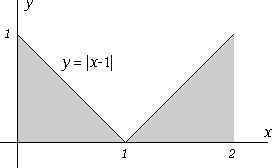
\includegraphics{01blooper1.pdf}}

\noindent%
Clearly the combined area of the two triangles should be 1.  Now let's try
to get this answer by integration.

Consider $\int_0^2 |x-1|\,\dd x$.  Let $f(x)=|x-1|$ so that
\[
f(x)=
\begin{cases}
  x-1 & \text{ if } x\geq 1\\
  1-x & \text{ if } x < 1\\
\end{cases}
\]
Define
\[
F(x)=
\begin{cases}
  \frac{1}{2}x^2-x & \text{ if } x\geq 1\\
  x-\frac{1}{2}x^2 & \text{ if } x < 1
\end{cases}
\]
Then since $F$ is an antiderivative of $f$ we have by the
Fundamental Theorem of Calculus:
\begin{align*}
  \int_0^2 |x-1|\,\dd x
  &=\int_0^2 f(x)\,\dd x\\
  &= F(2)-F(0)\\
  &=\Bigl(\frac{\;2^2}{2}-2\Bigr) - \Bigl(0-\frac{\;0^2}{2}\Bigr)\\
  &=0.
\end{align*}
But this integral cannot be zero, $f(x)$ is positive
except at one point.   How can this be?

\problem \textcolor{badgerred}{\itshape It turns out that the area enclosed by a %{{{3
circle is zero -- ?!}
According to the ancient formula for the area of a disc,  the
area of the following half-disc is $\pi/2$.

\noindent%
\raisebox{-80pt}{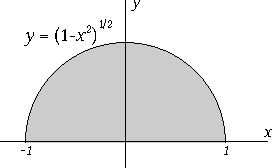
\includegraphics{01blooper2.pdf}}

We can also compute this area by means of an integral, namely
\[
\text{Area} = \int_{-1}^1 \sqrt{1-x^2}\;\dd x
\]
Substitute $u=1-x^2$ so: 
\begin{gather*}
  u=1-x^2,\quad
  x=\sqrt{1-u}=(1-u)^{\frac12},\\
  \dd x=(\frac12)(1-u)^{-\frac12}(-1)\;\dd u.
\end{gather*}
Hence
\begin{multline*}
  \int \sqrt{1-x^2}\;\dd x =\\
  \int \sqrt{u}\; (\frac12)(1-u)^{-\frac12}(-1)\;\dd u.
\end{multline*}
Now take the definite integral from $x=-1$ to $x=1$ and note that
$u=0$ when $x=-1$ and $u=0$ also when $x=1$, so
\begin{multline*}
  \int_{-1}^1 \sqrt{1-x^2}\;\dd x =\\
  \int_0^0 \sqrt{u} \bigl(\frac12\bigr)(1-u)^{-\frac12}(-1)\;\dd u=0
\end{multline*}
The last being zero since
\[
\int_0^0(\text{ anything })\;\dd x = 0.
\]
But the integral on the left is equal to half the area of the unit disc.
Therefore half a disc has zero area, and a whole disc should have twice
as much area: still zero!

How can this be?



\end{multicols}
\noproblemfont


%%% Local Variables:
%%% mode: latex
%%% TeX-master: "free222"
%%% End:
